% !TEX spellcheck = en_US



% ~~~~~~~~~~~~~~~~~~~~~~~~~~~~~~~~~~~~~~~ V
% (NC) 2026 Haluk Bingol
% github.com/halukbingol/LaTeX-Templates
%
% Licensees may copy, distribute, display, and perform the work and make derivative works 
% and remixes based on it only for non-commercial purposes. 
% ~~~~~~~~~~~~~~~~~~~~~~~~~~~~~~~~~~~~~~~ A




% =====================================================================
%  Stacks -- The Concepts
%  ---------------------------------------------------------------------
%  Built on hblib/Template/hblibTemplate.tex with the libraries in ../../hblib/.
%  Programs and their real outputs are in codeoutput/:
%     codeoutput/<Name>.java  a program (classes without main() are only compiled)
%     codeoutput/<Name>.sh    a terminal session, run in a copy of codeoutput/<Name>/
%     codeoutput/<Name>.txt   what it printed, made by:  bash run_examples.sh
% =====================================================================

\documentclass[aspectratio=169,10pt,compress]{beamer}

% ~~~~~~~~~~~~~~~~~~~~~~~~~~~~~~~~~~~~~~~~~~~~~~~~~~~~~~~~~~~~~~~~~ V hblib
	\usepackage{../../hblib/hblibPresentation} % lib presentation: theme, i/N, \hSection, algorithm2e, ...
	\usepackage{../../hblib/hblibCodeoutput} % lib code + output: \lstcode, \lstterminal, ...
	\usepackage{../../hblib/hblibDatastructures} % lib data structures: \hString, \hStack, \hQueue
% ~~~~~~~~~~~~~~~~~~~~~~~~~~~~~~~~~~~~~~~~~~~~~~~~~~~~~~~~~~~~~~~~~ A hblib


% xcolor, array (and the L{width} column), listings, tikz and algorithm2e come from the hblib libraries
\usepackage[T1]{fontenc}
\usepackage{lmodern}
\usepackage{booktabs}

\newcommand{\win}{\textbf{Windows}}
\newcommand{\mac}{\textbf{macOS}}

% algorithm2e set-up (the package is loaded by hblibPresentation)
\SetAlCapFnt{\small}
\SetAlCapNameFnt{\small}
\SetKwProg{Fn}{function}{}{end}
\SetKw{KwError}{error}

% ~~~~~~~~~~~~~~~~~~~~~~~~~~~~~~~~~~~~~~~ V title
\title[cis112 Stack as array]{
	{\small cis112}\\
	Stack
}

\subtitle{Stack as array}

\author[Bingol]{Haluk O. Bingol}

\institute[FCIS]{
    Faculty of Computer and Information Sciences\\
    Yeditepe University
}
\date{
	{\tiny \hbTimeStamp}
}
% ~~~~~~~~~~~~~~~~~~~~~~~~~~~~~~~~~~~~~~~ V title



\begin{document}




% ~~~~~~~~~~~~~~~~~~~~~~~~~~~~~~~~~~~~~~ V frm
\begin{frame}[t,fragile]
  \titlepage
\end{frame}
% ~~~~~~~~~~~~~~~~~~~~~~~~~~~~~~~~~~~~~~ A frm




% ~~~~~~~~~~~~~~~~~~~~~~~~~~~~~~~~~~~~~~ V frm
\begin{frame}[t,fragile] \frametitle{Outline}
  \begin{columns}[T]
    \begin{column}{0.35\textwidth}
      \tableofcontents[sections={1-4}, hideallsubsections]
    \end{column}
    \begin{column}{0.35\textwidth}
      \tableofcontents[sections={5-8}, hideallsubsections]
    \end{column}
    \begin{column}{0.30\textwidth}
%		\vspace{1cm}
		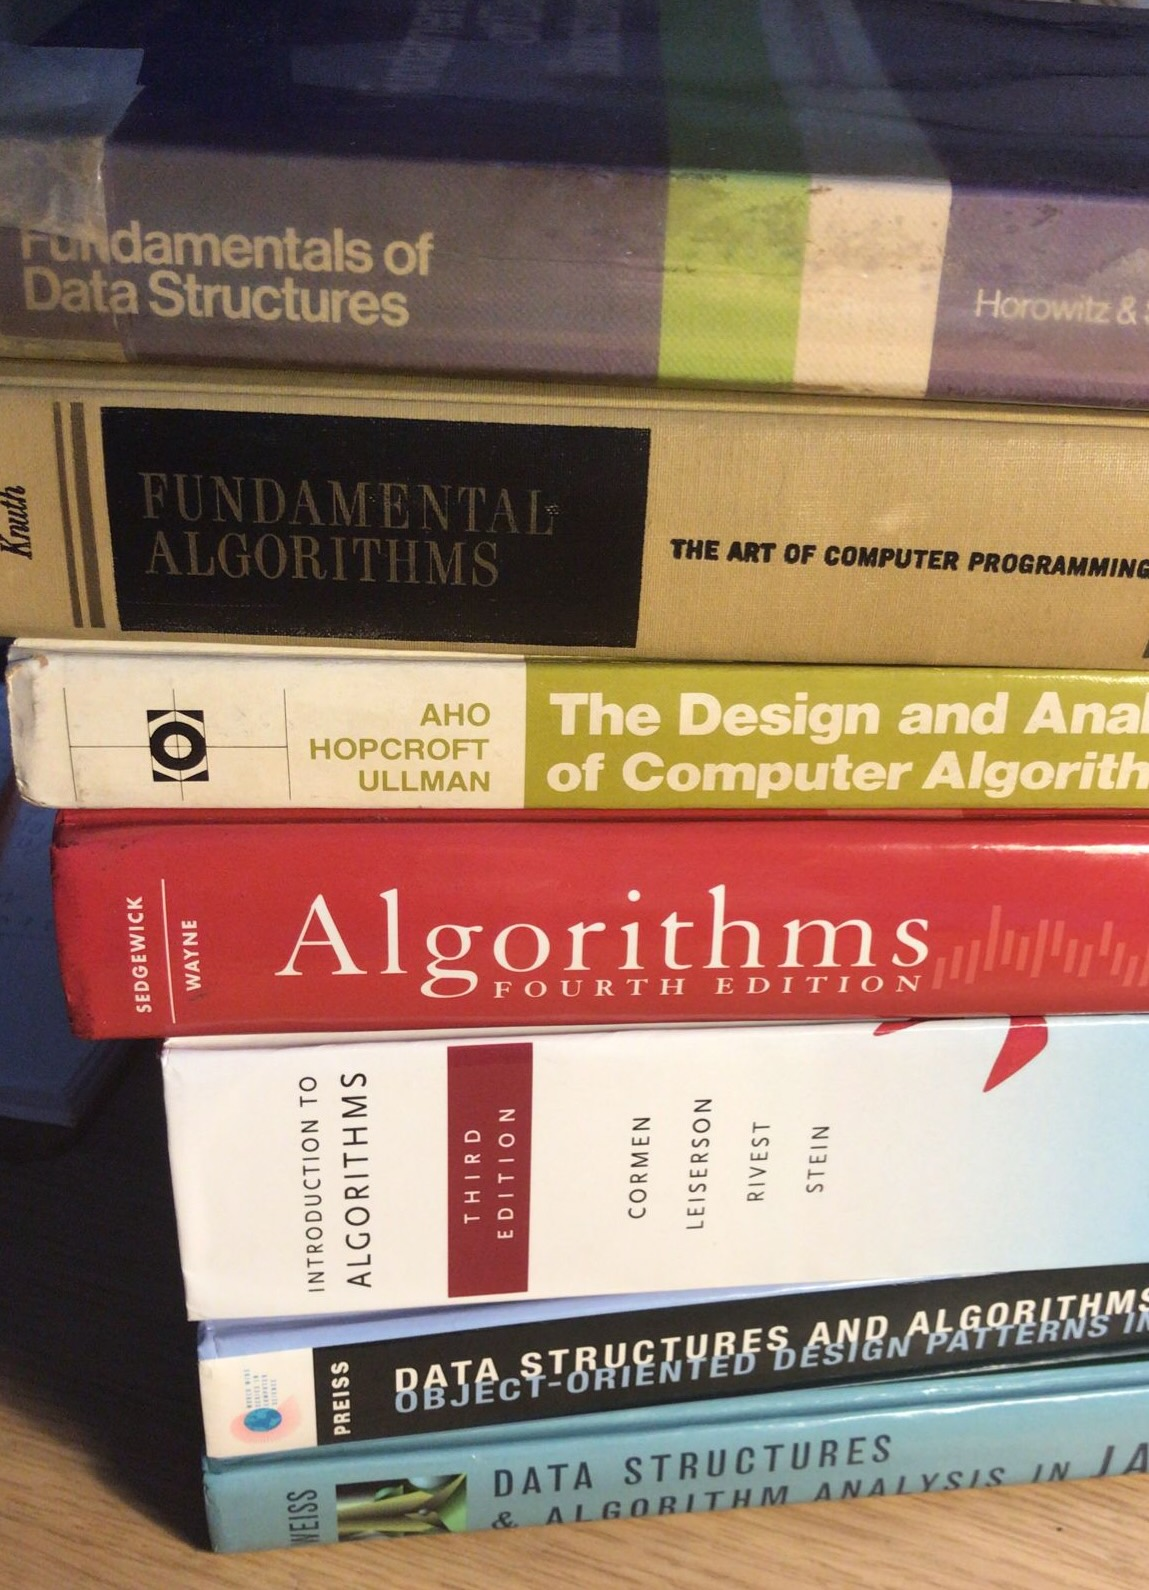
\includegraphics[width=.8\columnwidth]
			{fig-stackBooks.jpg}\\
		{\small Stack of books}
    \end{column}
  \end{columns}
\end{frame}
% ~~~~~~~~~~~~~~~~~~~~~~~~~~~~~~~~~~~~~~ A frm




% ~~~~~~~~~~~~~~~~~~~~~~~~~~~~~~~~~~~~~~ V
\hSection{Motivation}{}{}
% ~~~~~~~~~~~~~~~~~~~~~~~~~~~~~~~~~~~~~~ A




% ~~~~~~~~~~~~~~~~~~~~~~~~~~~~~~~~~~~~~~ V
\begin{frame}\frametitle{Motivation}

How does 

	\begin{itemize}

		\item 
		browser keep track of previous visited pages?

		\item 
		a text editor handle undo operations?

		\item 
		compiler check if the parentheses balanced?
		\begin{itemize}
			
			\item 
			Balanced: (),  (()),  ()(), (()((())))
			
			\item 
			Unbalanced: )(,  (())),  ())(), ((()((())))
			
		\end{itemize}

		\item 
		evaluate expression
		\begin{itemize}
			
			\item 
			1 + 2 * 3
			
		\end{itemize}
	\end{itemize}
\end{frame}
% ~~~~~~~~~~~~~~~~~~~~~~~~~~~~~~~~~~~~~~ A




% ~~~~~~~~~~~~~~~~~~~~~~~~~~~~~~~~~~~~~~ V
\hSection{Case: Browser visiting pages}{}{}
% ~~~~~~~~~~~~~~~~~~~~~~~~~~~~~~~~~~~~~~ A




% ~~~~~~~~~~~~~~~~~~~~~~~~~~~~~~~~~~~~~~ V
\begin{frame}\frametitle{Case: Browser visiting pages}

\begingroup
\setlength{\tabcolsep}{3pt}
\renewcommand{\arraystretch}{.1}
\begin{center}
\begin{tabular}{l l l}

	%
	\textbf{Visit page} &\textbf{Page seen}
	&\textbf{History}\\
	%
	\pause
	A &A
	&\begin{tikzpicture}
		\hStack{0}{4}{0}{A, , , }[0.5][0.5]
	\end{tikzpicture}\\
	%
	\pause
	B &B
	&\begin{tikzpicture}
		\hStack{0}{4}{1}{A, B, , }[0.5][0.5]
	\end{tikzpicture}\\
	%
	\pause
	C &C
	&\begin{tikzpicture}
		\hStack{0}{4}{2}{A, B, C, }[0.5][0.5]
	\end{tikzpicture}\\
	%
	\pause
	Back &B
	&\begin{tikzpicture}
		\hStack{0}{4}{1}{A, B, C, }[0.5][0.5]
	\end{tikzpicture}
	{\tiny C is still there!}\\
	%
	\pause
	Back &A
	&\begin{tikzpicture}
		\hStack{0}{4}{0}{A, B, C, }[0.5][0.5]
	\end{tikzpicture}
	{\tiny what if we back once more?}\\
	%
	\pause
	D &D
	&\begin{tikzpicture}
		\hStack{0}{4}{1}{A, D, C, }[0.5][0.5]
	\end{tikzpicture}\\
	%
	\pause
	E &E
	&\begin{tikzpicture}
		\hStack{0}{4}{2}{A, D, E, }[0.5][0.5]
	\end{tikzpicture}\\
	%
	\pause
	F &F
	&\begin{tikzpicture}
		\hStack{0}{4}{3}{A, D, E, F}[0.5][0.5]
	\end{tikzpicture}
	{\tiny what if we visit one more page?}\\
	%
	\pause
	Back &E
	&\begin{tikzpicture}
		\hStack{0}{4}{2}{A, D, E, F}[0.5][0.5]
	\end{tikzpicture}\\


\end{tabular}
\end{center}
\endgroup
\end{frame}
% ~~~~~~~~~~~~~~~~~~~~~~~~~~~~~~~~~~~~~~ A




%% ~~~~~~~~~~~~~~~~~~~~~~~~~~~~~~~~~~~~~~ V
%\begin{frame}\frametitle{Case: Browser visiting pages}
%
%	\begin{columns}[T] % >>>>
%	\begin{column}{.3\linewidth} % ++++ V visits
%	    	\textbf{Visit page}
%	\end{column} % ++++ A
%	\begin{column}{.2\linewidth} % ++++ V seen
%		\textbf{Page seen}
%	\end{column} % ++++ A
%	\begin{column}{.5\linewidth} % ++++ V history
%	    	\textbf{History}
%	\end{column} % ++++ A
%	\end{columns} % <<<<
%	
%%	\pause
%%	\vspace{0.08cm}	
%	\begin{columns}[T] % >>>>
%	\begin{column}{.3\linewidth} % ++++ V visits
%	    	P1
%	\end{column} % ++++ A
%	\begin{column}{.2\linewidth} % ++++ V seen
%		P1
%	\end{column} % ++++ A
%	\begin{column}{.5\linewidth} % ++++ V history
%		\begin{tikzpicture}
%			\hStack{0}{4}{1}{P1}[0.8][0.28]
%		\end{tikzpicture}
%	\end{column} % ++++ A
%	\end{columns} % <<<<
%	
%	\pause
%	\vspace{0.08cm}	
%	\begin{columns}[T] % >>>>
%	\begin{column}{.3\linewidth} % ++++ V visits
%	    	P2
%	\end{column} % ++++ A
%	\begin{column}{.2\linewidth} % ++++ V seen
%		P2
%	\end{column} % ++++ A
%	\begin{column}{.5\linewidth} % ++++ V history
%		\begin{tikzpicture}
%			\hStack{0}{4}{2}{P1, P2}[0.8][0.28]
%		\end{tikzpicture}
%	\end{column} % ++++ A
%	\end{columns} % <<<<
%	
%	\pause
%	\vspace{0.08cm}	
%	\begin{columns}[T] % >>>>
%	\begin{column}{.3\linewidth} % ++++ V visits
%	    	P3
%	\end{column} % ++++ A
%	\begin{column}{.2\linewidth} % ++++ V seen
%		P3
%	\end{column} % ++++ A
%	\begin{column}{.5\linewidth} % ++++ V history
%		\begin{tikzpicture}
%			\hStack{0}{4}{3}{P1, P2, P3}[0.8][0.28]
%		\end{tikzpicture}
%	\end{column} % ++++ A
%	\end{columns} % <<<<
%	
%	\pause
%	\vspace{0.08cm}	
%	\begin{columns}[T] % >>>>
%	\begin{column}{.3\linewidth} % ++++ V visits
%	    	Back
%	\end{column} % ++++ A
%	\begin{column}{.2\linewidth} % ++++ V seen
%		P2
%	\end{column} % ++++ A
%	\begin{column}{.5\linewidth} % ++++ V history
%		\begin{tikzpicture}
%			\hStack{0}{4}{2}{P1, P2, P3}[0.8][0.28]
%		\end{tikzpicture}
%		{\scriptsize P3 not deleted}
%	\end{column} % ++++ A
%	\end{columns} % <<<<
%	
%	\pause
%	\vspace{0.08cm}	
%	\begin{columns}[T] % >>>>
%	\begin{column}{.3\linewidth} % ++++ V visits
%	    	Back
%	\end{column} % ++++ A
%	\begin{column}{.2\linewidth} % ++++ V seen
%		P1
%	\end{column} % ++++ A
%	\begin{column}{.5\linewidth} % ++++ V history
%		\begin{tikzpicture}
%			\hStack{0}{4}{1}{P1, P2, P3}[0.8][0.28]
%		\end{tikzpicture}
%	\end{column} % ++++ A
%	\end{columns} % <<<<
%	
%	\pause
%	\vspace{0.08cm}	
%	\begin{columns}[T] % >>>>
%	\begin{column}{.3\linewidth} % ++++ V visits
%	    	P4
%	\end{column} % ++++ A
%	\begin{column}{.2\linewidth} % ++++ V seen
%		P4
%	\end{column} % ++++ A
%	\begin{column}{.5\linewidth} % ++++ V history
%		\begin{tikzpicture}
%			\hStack{0}{4}{2}{P1, P4, P3}[0.8][0.28]
%		\end{tikzpicture}
%	\end{column} % ++++ A
%	\end{columns} % <<<<
%	
%	\pause
%	\vspace{0.08cm}	
%	\begin{columns}[T] % >>>>
%	\begin{column}{.3\linewidth} % ++++ V visits
%	    	P5
%	\end{column} % ++++ A
%	\begin{column}{.2\linewidth} % ++++ V seen
%		P5
%	\end{column} % ++++ A
%	\begin{column}{.5\linewidth} % ++++ V history
%		\begin{tikzpicture}
%			\hStack{0}{4}{3}{P1, P4, P5}[0.8][0.28]
%		\end{tikzpicture}
%	\end{column} % ++++ A
%	\end{columns} % <<<<
%	
%	\pause
%	\vspace{0.08cm}	
%	\begin{columns}[T] % >>>>
%	\begin{column}{.3\linewidth} % ++++ V visits
%	    	P6
%	\end{column} % ++++ A
%	\begin{column}{.2\linewidth} % ++++ V seen
%		P6
%	\end{column} % ++++ A
%	\begin{column}{.5\linewidth} % ++++ V history
%		\begin{tikzpicture}
%			\hStack{0}{4}{4}{P1, P4, P5, P6}[0.8][0.28]
%		\end{tikzpicture}
%	\end{column} % ++++ A
%	\end{columns} % <<<<
%	
%	\pause
%	\vspace{0.08cm}	
%	\begin{columns}[T] % >>>>
%	\begin{column}{.3\linewidth} % ++++ V visits
%	    	Back
%	\end{column} % ++++ A
%	\begin{column}{.2\linewidth} % ++++ V seen
%		P5
%	\end{column} % ++++ A
%	\begin{column}{.5\linewidth} % ++++ V history
%		\begin{tikzpicture}
%			\hStack{0}{4}{3}{P1, P4, P5, P6}[0.8][0.28]
%		\end{tikzpicture}
%	\end{column} % ++++ A
%	\end{columns} % <<<<
%	
%	\pause
%	\vspace{0.08cm}
%	\begin{columns}[T] % >>>>
%	\begin{column}{.3\linewidth} % ++++ V visits
%	    	Back
%	\end{column} % ++++ A
%	\begin{column}{.2\linewidth} % ++++ V seen
%		P4
%	\end{column} % ++++ A
%	\begin{column}{.5\linewidth} % ++++ V history
%		\begin{tikzpicture}
%			\hStack{0}{4}{2}{P1, P4, P5, P6}[0.8][0.28]
%		\end{tikzpicture}
%	\end{column} % ++++ A
%	\end{columns} % <<<<
%
%\end{frame}
%% ~~~~~~~~~~~~~~~~~~~~~~~~~~~~~~~~~~~~~~ A




% ~~~~~~~~~~~~~~~~~~~~~~~~~~~~~~~~~~~~~~ V
\hSection{Implementation}{}{}
% ~~~~~~~~~~~~~~~~~~~~~~~~~~~~~~~~~~~~~~ A




% ~~~~~~~~~~~~~~~~~~~~~~~~~~~~~~~~~~~~~~ V
\begin{frame}\frametitle{Observations}
	\begin{columns}[T] % >>>>
	\begin{column}{.5\linewidth} % ++++ V
		\begin{itemize}
			\item
			\hEmph{insert(item)}
				\begin{itemize}
					\item 
					at  \hEmph{lastUsedLocation} + 1
				\end{itemize}			

			\item
			\hEmph{delete()}
				\begin{itemize}
					\item 
					at  \hEmph{lastUsedLocation}
				\end{itemize}			
			\item
			Use array
				\begin{itemize}
					\item 
					keep track of  \hEmph{lastUsedLocation}
				\end{itemize}			
		\end{itemize}
	\end{column} % ++++ A
	\begin{column}{.5\linewidth} % ++++ V
	
		\vspace{-1cm}
	    	\textbf{History}\\
		%
		\begin{tikzpicture}
			\hStack{0}{4}{0}{A, , , }[0.5][0.5]
		\end{tikzpicture}\\
		%
		\begin{tikzpicture}
			\hStack{0}{4}{1}{A, B, , }[0.5][0.5]
		\end{tikzpicture}\\
		%
		\begin{tikzpicture}
			\hStack{0}{4}{2}{A, B, C, }[0.5][0.5]
		\end{tikzpicture}\\
		%
		\begin{tikzpicture}
			\hStack{0}{4}{1}{A, B, C, }[0.5][0.5]
		\end{tikzpicture}\\
		%
		\begin{tikzpicture}
			\hStack{0}{4}{0}{A, B, C, }[0.5][0.5]
		\end{tikzpicture}\\
		%
		\begin{tikzpicture}
			\hStack{0}{4}{1}{A, D, C, }[0.5][0.5]
		\end{tikzpicture}\\
		%
		\begin{tikzpicture}
			\hStack{0}{4}{2}{A, D, E, }[0.5][0.5]
		\end{tikzpicture}\\
		%
		\begin{tikzpicture}
			\hStack{0}{4}{3}{A, D, E, F}[0.5][0.5]
		\end{tikzpicture}\\
		%
		\begin{tikzpicture}
			\hStack{0}{4}{2}{A, D, E, F}[0.5][0.5]
		\end{tikzpicture}\\

	\end{column} % ++++ A
	\end{columns} % <<<<
\end{frame}
% ~~~~~~~~~~~~~~~~~~~~~~~~~~~~~~~~~~~~~~ A




% ~~~~~~~~~~~~~~~~~~~~~~~~~~~~~~~~~~~~~~ V
\begin{frame}\frametitle{Implementation with array}
	\begin{columns}[T] % >>>>
	\begin{column}{.5\linewidth} % ++++ V
		\begin{itemize}
			\item
			\hEmph{push(item)} \sout{insert(item)}
				\begin{itemize}
					\item 
					at  \hEmph{top + 1}
					\sout{lastUsedLocation + 1}
				\end{itemize}			

			\item
			\hEmph{pop()} \sout{delete(item)}
				\begin{itemize}
					\item 
					at \hEmph{top}
					\sout{lastUsedLocation}
				\end{itemize}			
			\item
			Use array
				\begin{itemize}
					\item 
					keep track of  \hEmph{top} 
					\sout{lastUsedLocation} 
				\end{itemize}			
		\end{itemize}
		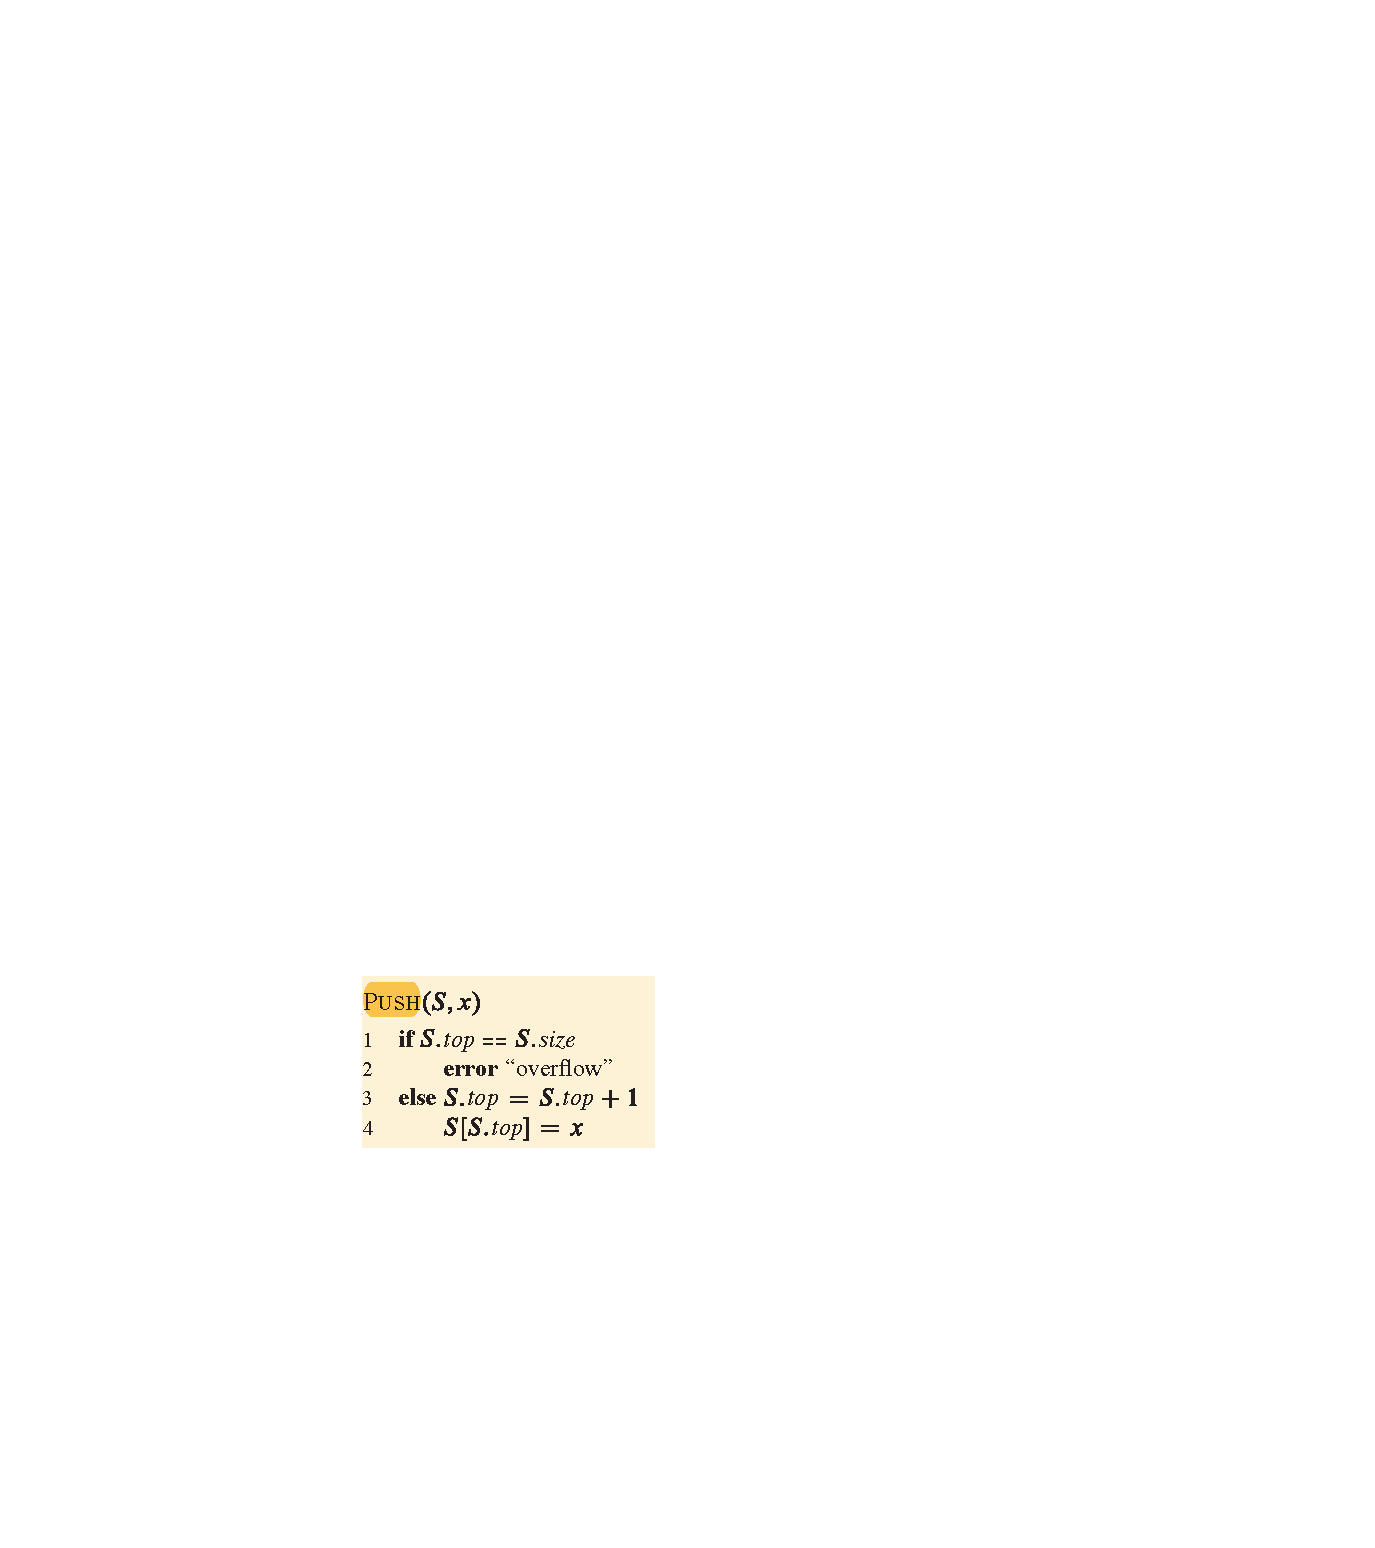
\includegraphics[width=.4\columnwidth]
			{fig-stack-push.pdf}
		\quad
		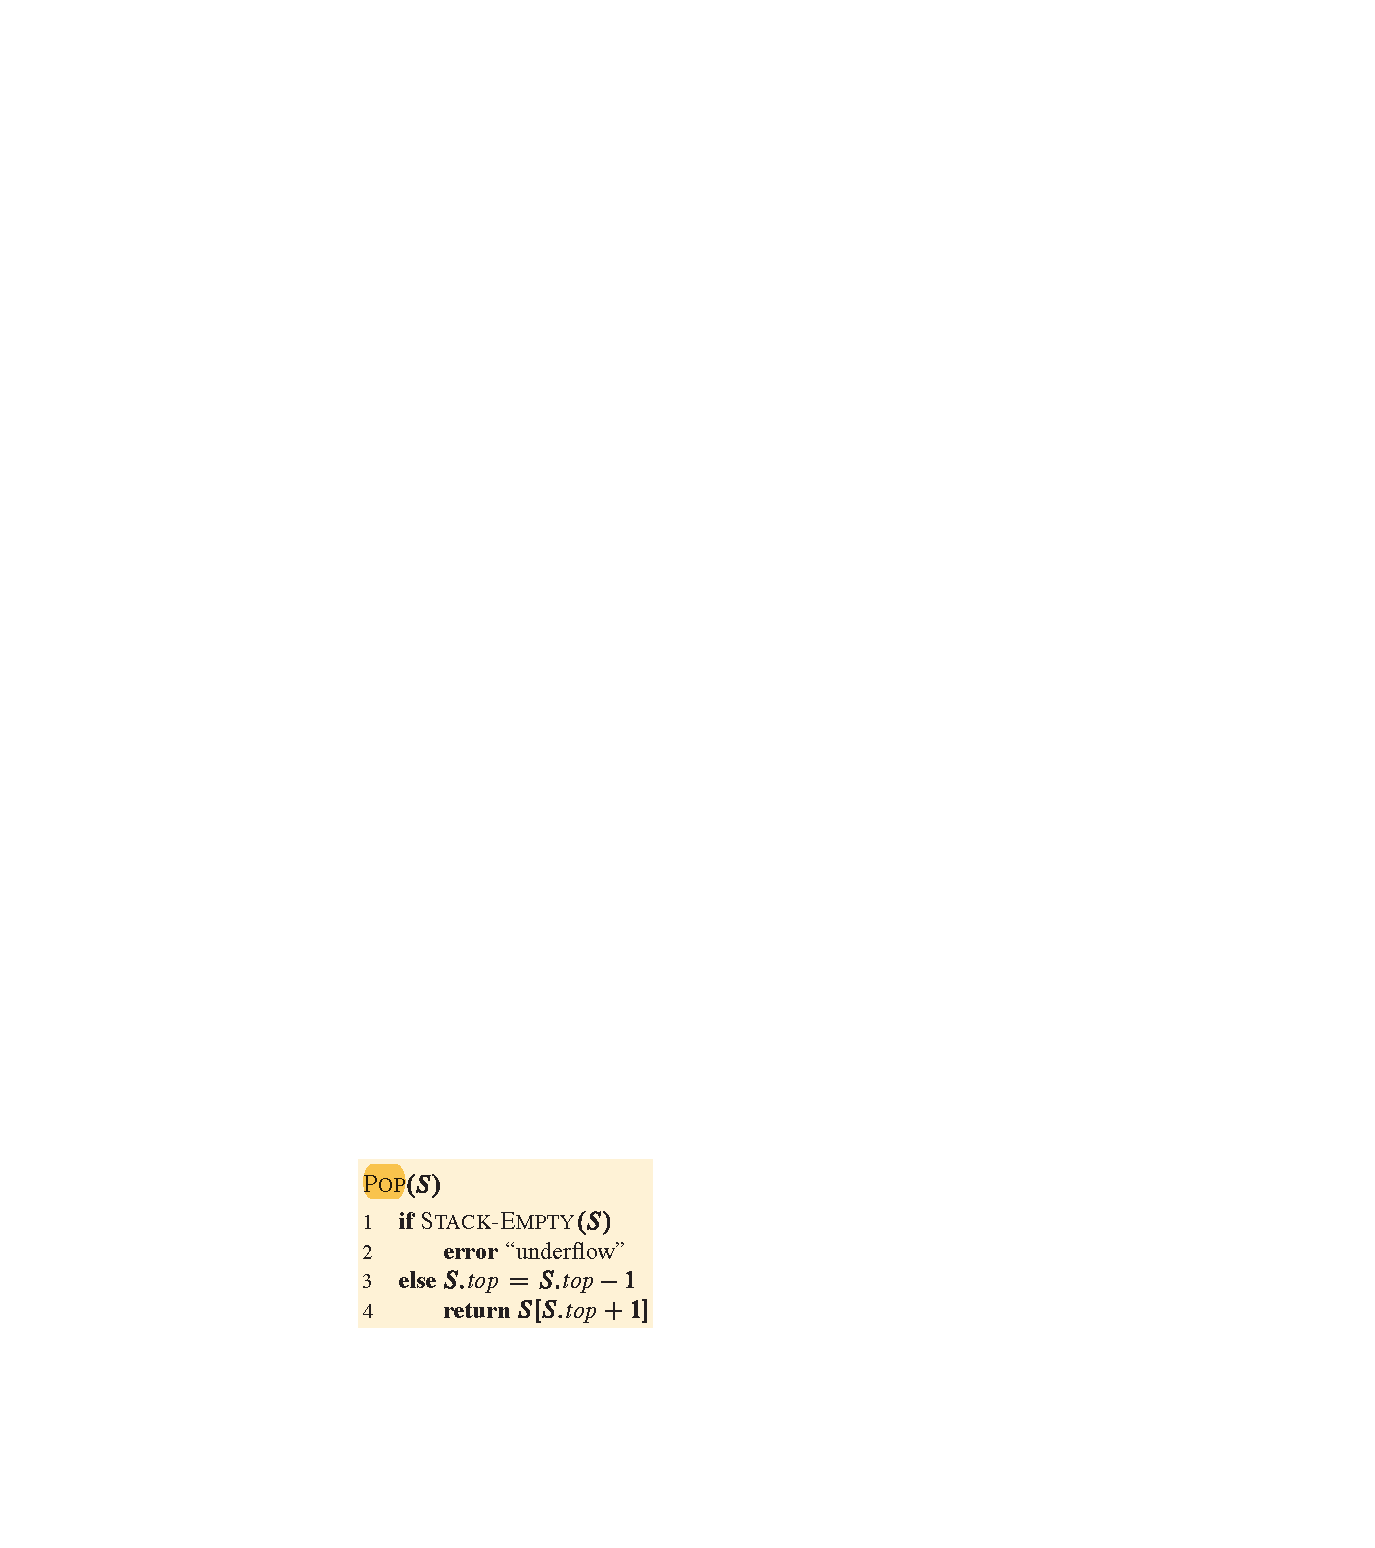
\includegraphics[width=.4\columnwidth]
			{fig-stack-pop.pdf}
		\\
		\vspace{0.2cm}	
		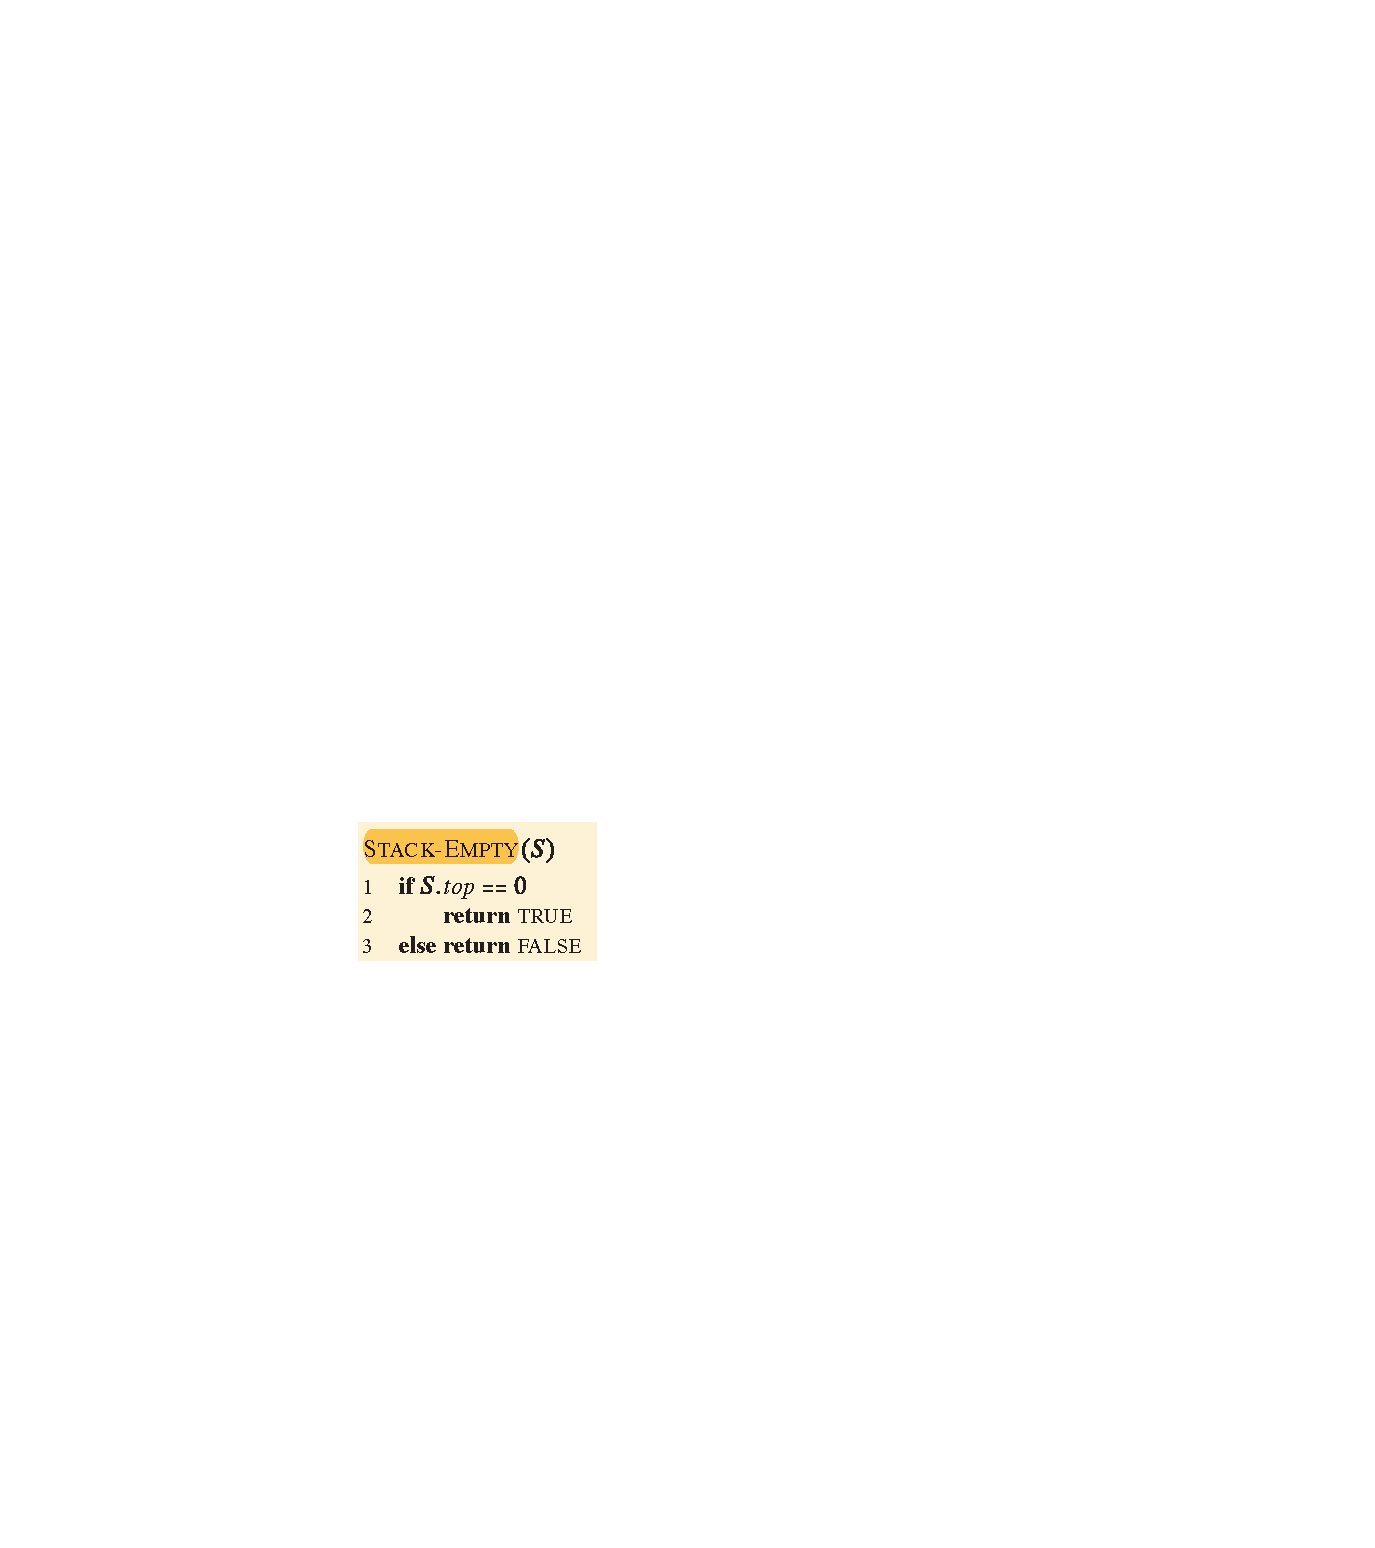
\includegraphics[width=.4\columnwidth]
			{fig-stack-empty.pdf}			
		\hCite{%
			source: CLRS~\cite{cormen2022introduction}
		}
		
		\hCite{%
			\cite{cormen2022introduction},%
			\cite{aho1974design},%
			\cite{horowitz1982fundamentals},%
			\cite{horstmann2016big}
		}
					
	\end{column} % ++++ A
	\begin{column}{.5\linewidth} % ++++ V

	\vspace{-1cm}
	    	\textbf{Array}\\
		%
		\begin{tikzpicture}
			\hStack{0}{4}{0}{A, , , }[0.5][0.5]
		\end{tikzpicture}\\
		%
		\begin{tikzpicture}
			\hStack{0}{4}{1}{A, B, , }[0.5][0.5]
		\end{tikzpicture}\\
		%
		\begin{tikzpicture}
			\hStack{0}{4}{2}{A, B, C, }[0.5][0.5]
		\end{tikzpicture}\\
		%
		\begin{tikzpicture}
			\hStack{0}{4}{1}{A, B, C, }[0.5][0.5]
		\end{tikzpicture}\\
		%
		\begin{tikzpicture}
			\hStack{0}{4}{0}{A, B, C, }[0.5][0.5]
		\end{tikzpicture}\\
		%
		\begin{tikzpicture}
			\hStack{0}{4}{1}{A, D, C, }[0.5][0.5]
		\end{tikzpicture}\\
		%
		\begin{tikzpicture}
			\hStack{0}{4}{2}{A, D, E, }[0.5][0.5]
		\end{tikzpicture}\\
		%
		\begin{tikzpicture}
			\hStack{0}{4}{3}{A, D, E, F}[0.5][0.5]
		\end{tikzpicture}\\
		%
		\begin{tikzpicture}
			\hStack{0}{4}{2}{A, D, E, F}[0.5][0.5]
		\end{tikzpicture}\\

	\end{column} % ++++ A
	\end{columns} % <<<<
\end{frame}
% ~~~~~~~~~~~~~~~~~~~~~~~~~~~~~~~~~~~~~~ A




% ~~~~~~~~~~~~~~~~~~~~~~~~~~~~~~~~~~~~~~ V
\hSection{Abstraction}{Abstract Data Types (ADT)}{}
% ~~~~~~~~~~~~~~~~~~~~~~~~~~~~~~~~~~~~~~ A




% ~~~~~~~~~~~~~~~~~~~~~~~~~~~~~~~~~~~~~~ V
\hSubsection{Abstraction-ADT}{Container}{}
% ~~~~~~~~~~~~~~~~~~~~~~~~~~~~~~~~~~~~~~ A




% ~~~~~~~~~~~~~~~~~~~~~~~~~~~~~~~~~~~~~~ V
\begin{frame}\frametitle{Abstraction-ADT: \hEmph{Container}}
	\begin{columns}[T] % >>>>
	\begin{column}{.5\linewidth} % ++++ V
	    	Container: contains items
		\begin{itemize}
			\item \hEmph{insert}(item)
			\item \hEmph{delete}(item)
			\item \hEmph{isIn}(item)
			\item \hEmph{isEmpty}()
			\item \hEmph{isFull}()
			\item \hEmph{size}()			
		\end{itemize}
	\end{column} % ++++ A
	\begin{column}{.5\linewidth} % ++++ V
		\begin{itemize}

			\item
			Insertion
			\begin{itemize}
				\item
				Order of is \hEmph{not} important
	
				\item
				Duplication is allowed
			\end{itemize}

			\item
			Deletion
			\begin{itemize}
				\item
				Any item can be deleted
			\end{itemize}
		\end{itemize}
	\end{column} % ++++ A
	\end{columns} % <<<<
\end{frame}
% ~~~~~~~~~~~~~~~~~~~~~~~~~~~~~~~~~~~~~~ A




% ~~~~~~~~~~~~~~~~~~~~~~~~~~~~~~~~~~~~~~ V
\hSubsection{Abstraction-ADT}{Set}{}
% ~~~~~~~~~~~~~~~~~~~~~~~~~~~~~~~~~~~~~~ A




% ~~~~~~~~~~~~~~~~~~~~~~~~~~~~~~~~~~~~~~ V
\begin{frame}\frametitle{Abstraction-ADT: \hEmph{Set}}
	\begin{columns}[T] % >>>>
	\begin{column}{.5\linewidth} % ++++ V
	    	Container: contains items
		\begin{itemize}
			\item insert(item)
			\item delete(item)
			\item isIn(item)
			\item isEmpty()
			\item isFull()
			\item size()			
		\end{itemize}
	\end{column} % ++++ A
	\begin{column}{.5\linewidth} % ++++ V
		\begin{itemize}

			\item
			Insertion
			\begin{itemize}
				\item
				Order of is \hEmph{not} important
	
				\item
				Duplication is  \hEmph{not} allowed
			\end{itemize}

			\item
			Deletion
			\begin{itemize}
				\item
				Any item can be deleted
			\end{itemize}
		\end{itemize}
	\end{column} % ++++ A
	\end{columns} % <<<<
\end{frame}
% ~~~~~~~~~~~~~~~~~~~~~~~~~~~~~~~~~~~~~~ A




% ~~~~~~~~~~~~~~~~~~~~~~~~~~~~~~~~~~~~~~ V
\hSubsection{Abstraction-ADT}{Stack}{}
% ~~~~~~~~~~~~~~~~~~~~~~~~~~~~~~~~~~~~~~ A




% ~~~~~~~~~~~~~~~~~~~~~~~~~~~~~~~~~~~~~~ V
\begin{frame}\frametitle{Abstraction-ADT: \hEmph{Stack}}
	\begin{columns}[T] % >>>>
	\begin{column}{.5\linewidth} % ++++ V
	    	Container: contains items
		\begin{itemize}
			\item \hEmph{push}(item) \sout{insert(item)}
			\item \hEmph{pop()} \sout{delete(item)}
			\item \sout{isIn(item)}
			\item \hEmph{isEmpty}()
			\item \hEmph{isFull}()
			\item \sout{size()}			
		\end{itemize}
	\end{column} % ++++ A
	\begin{column}{.5\linewidth} % ++++ V
		\begin{itemize}

			\item
			\hEmph{Last-In-First-Out} (\hEmph{LIFO})

			\item
			Insertion
			\begin{itemize}
				\item
				Order of is \hEmph{important} 
	
				\item
				Duplication is \hEmph{allowed}
			\end{itemize}

			\item
			Deletion
			\begin{itemize}
				\item
				\sout{Any item can be deleted}
				
				\item
				Only a \hEmph{specific} item can be deleted
			\end{itemize}
		\end{itemize}
	\end{column} % ++++ A
	\end{columns} % <<<<
\end{frame}
% ~~~~~~~~~~~~~~~~~~~~~~~~~~~~~~~~~~~~~~ A




% ~~~~~~~~~~~~~~~~~~~~~~~~~~~~~~~~~~~~~~ V
\hSection{Applications}{}{}
% ~~~~~~~~~~~~~~~~~~~~~~~~~~~~~~~~~~~~~~ A




% ~~~~~~~~~~~~~~~~~~~~~~~~~~~~~~~~~~~~~~ V
\hSubsection{Applications}{Balanced parentheses}{}
% ~~~~~~~~~~~~~~~~~~~~~~~~~~~~~~~~~~~~~~ A




% ~~~~~~~~~~~~~~~~~~~~~~~~~~~~~~~~~~~~~~ V
\begin{frame}\frametitle{Balanced Parentheses}
	\begin{columns}[T] % >>>>
	\begin{column}{.5\linewidth} % ++++ V
{\tiny 
\begin{algorithm}[H]
	\SetKwData{Stack}{\texttt{stack}}
	\SetKwData{Ch}{\texttt{ch}}
	\SetKwData{Cs}{\texttt{cs}}
	\KwData{algebraic expression}
	\KwResult{true if parentheses are balanced}
	\Begin{
		\ForEach {\Ch in expression from left to right} {
		
			\If {\Ch is an opening parenthesis} {
				push \Ch on the \Stack
			}\ElseIf {\Ch is a closing parenthesis} {
				\Cs $\leftarrow$ pop the \Stack \\
				\If {the opening \Cs and closing \Ch parentheses don’t match} {
					\Return FALSE 
				}
			}
		}
		\If {at the end the \Stack is empty} {
			\Return TRUE 
		} \Else {
			\Return FALSE
		}
	    
		\caption{{\footnotesize Balanced Parentheses}}
	}
\end{algorithm}
} % \tiny

\hCite{Horstmann~\cite{horstmann2016big}}

	\end{column} % ++++ A
	\begin{column}{.5\linewidth} % ++++ V
	
	\vspace{-1cm}
{\tiny
	expression: (~)~(~(~(~)~(~)~)~)\\
	\begin{center}
	\begin{tabular}{l l}
		\textbf{ch}
		&\textbf{stack}\\
		
		(
		&\begin{tikzpicture}
			\hStack{0}{4}{0}{``(''} [0.5][0.5]
		\end{tikzpicture}\\			
		
		)
		&\begin{tikzpicture}
			\hStack{0}{4}{-1}{} [0.5][0.5]
		\end{tikzpicture}\\			
		
		(
		&\begin{tikzpicture}
			\hStack{0}{4}{0}{``(''} [0.5][0.5]
		\end{tikzpicture}\\			
		
		(
		&\begin{tikzpicture}
			\hStack{0}{4}{1}{``('', ``(''} [0.5][0.5]
		\end{tikzpicture}\\			
		
		(
		&\begin{tikzpicture}
			\hStack{0}{4}{2}{``('', ``('', ``(''} [0.5][0.5]
		\end{tikzpicture}\\			
		
		)
		&\begin{tikzpicture}
			\hStack{0}{4}{1}{``('', ``(''} [0.5][0.5]
		\end{tikzpicture}\\			
		
		(
		&\begin{tikzpicture}
			\hStack{0}{4}{2}{``('', ``('', ``(''} [0.5][0.5]
		\end{tikzpicture}\\			
		
		)
		&\begin{tikzpicture}
			\hStack{0}{4}{1}{``('', ``(''} [0.5][0.5]
		\end{tikzpicture}\\			
		
		)
		&\begin{tikzpicture}
			\hStack{0}{4}{0}{``(''} [0.5][0.5]
		\end{tikzpicture}\\			
		
		)
		&\begin{tikzpicture}
			\hStack{0}{4}{-1}{} [0.5][0.5]
		\end{tikzpicture}
		{\small \hEmph{~~ Balanced}}\\			

	\end{tabular}
\end{center}
} % \tiny
	\end{column} % ++++ A
	\end{columns} % <<<<
\end{frame}
% ~~~~~~~~~~~~~~~~~~~~~~~~~~~~~~~~~~~~~~ A




%% ~~~~~~~~~~~~~~~~~~~~~~~~~~~~~~~~~~~~~~ V
%\begin{frame}\frametitle{Balanced Tags}
%	\lstset{
%		language=xml,
%		tabsize=3,
%		%frame=lines,
%%		caption=Test,
%		label=code:sample,
%		frame=shadowbox,
%		rulesepcolor=\color{gray},
%		xleftmargin=20pt,
%		framexleftmargin=15pt,
%		keywordstyle=\color{blue},
%		commentstyle=\color{darkgreen},
%		stringstyle=\color{red},
%%		numbers=left,
%%		numberstyle=\tiny,
%%		numbersep=5pt,
%		breaklines=true,
%		showstringspaces=false,
%		basicstyle=\tiny,
%		stringstyle=\color{blue},
%		emph={html,head,title,body,note,to,from,heading},emphstyle={\color{magenta}}
%	}
%	\begin{itemize}
%		
%		\item 
%		\hEmph{Arithmetic expressions}
%		\begin{itemize}			
%			\item 
%			$[a+b]*(c-d)$
%		\end{itemize}
%	
%		\item 
%		\hEmph{HTML tags}
%		\lstinputlisting{code-sample-html.html}
%		
%		\item 
%		\hEmph{XML tags}
%		\lstinputlisting{code-sample-xml.xml}
%	\end{itemize}
%
%\end{frame}
%% ~~~~~~~~~~~~~~~~~~~~~~~~~~~~~~~~~~~~~~ A




% ~~~~~~~~~~~~~~~~~~~~~~~~~~~~~~~~~~~~~~ V
\hSubsection{Applications}{Postfix Evaluation}{}
% ~~~~~~~~~~~~~~~~~~~~~~~~~~~~~~~~~~~~~~ A




% ~~~~~~~~~~~~~~~~~~~~~~~~~~~~~~~~~~~~~~ V
\begin{frame}\frametitle{Infix, Prefix, and Postfix (RPN) Notations}
% https://www.calcont.in/Conversion/infix_to_prefix
\begin{center}
\begin{tabular}{l l l}
	\textbf{infix notation} 
	&\textbf{prefix notation} 
	&\textbf{postfix notation}\\
	%
	{\tiny normal math expression} 
	&{\tiny operators followed by operands} 
	&{\tiny operands followed by operators}\\
	%
	$a + b$
	&$+ a~b$
	&$a~b +$\\
	%
	$a+b+c$
	&$+a + b~c$
	&$a~b + c +$\\
	%
	$a + b * c$
	&$+ a * b~c$
	&$a~b~c*+$\\
	%
	$(a + b) * c$
	&$*+a~b~c$
	&$a~b+c*$\\
	%
	$a+b*c/(e-f)$
	&$+a~/*b~c-e~f$
	&$a~b~c*e~f-/+$\\
	%
	~
	&~
	&	\hCite{
		\href
			{https://hp15c.com/web/hp15c.html}
			{HP-15 calculator online}~\cite{hp15online}
	}
\end{tabular}
\end{center}

	\vspace{1cm}
	Postfix notation is also called  
		\href
			{https://en.wikipedia.org/wiki/Reverse_Polish_notation}
			{\hEmph{Reverse Polish Notation (RPN)}}~\cite{wikipediaRPN}
	

	\hCite{%
		\href
			{https://www.openbookproject.net/books/pythonds/BasicDS/InfixPrefixandPostfixExpressions.html}
			{Infix, Prefix and Postfix Expressions}~\cite{pswadsPostfix}	
	}\\
	\hCite{%
		\href
			{https://www.web4college.com/converters/infix-to-postfix-prefix.php}
			{Infix to Postfix/Prefix converter}
	}

\end{frame}
% ~~~~~~~~~~~~~~~~~~~~~~~~~~~~~~~~~~~~~~ A




% ~~~~~~~~~~~~~~~~~~~~~~~~~~~~~~~~~~~~~~ V
\begin{frame}\frametitle{RPN Evaluation}
	\begin{columns}[T] % >>>>
	\begin{column}{.4\linewidth} % ++++ V
{\tiny 


% +++++++++++++++++++++++++++++++++++++++ V
%: -Alg. 
\begin{algorithm}[H]
	\SetKwData{Stack}{\texttt{stack}}
	\KwData{postfix expression}
	\KwResult{value of the expression}
	\Begin{
		\While {there is a token}{
			\If{an operator is read} {
				Pop two values off the \Stack\\
				Apply the operator to the two values \\
				Push the result back onto the \Stack
			} \ElseIf{a number is read} {
				Push it on the \Stack
			} 
		}
		Pop and display the result
	\caption{{\footnotesize RPN Evaluation}}
	}
\end{algorithm}
% +++++++++++++++++++++++++++++++++++++++ A

}

\hCite{Horstmann~\cite{horstmann2016big}}\\
\hCite{
	\href
		{https://hp15c.com/web/hp15c.html}
		{HP-15 calculator online}~\cite{hp15online}
}


	\end{column} % ++++ A
	\begin{column}{.4\linewidth} % ++++ V
	
		\vspace{-1cm}
		Use one stack\\
{\tiny
\begin{center}
	\begin{tabular}{l l}
		%
		\textbf{token}
		&\textbf{stack}\\
		%
		3
		&\begin{tikzpicture}
			\hStack{0}{5}{0}{3} [0.5][0.5]
		\end{tikzpicture}\\
		%
		4
		&\begin{tikzpicture}
			\hStack{0}{5}{1}{3, 4} [0.5][0.5]
		\end{tikzpicture}\\
		%
		+
		&\begin{tikzpicture}
			\hStack{0}{5}{0}{7} [0.5][0.5]
		\end{tikzpicture}\\
		%
		5
		&\begin{tikzpicture}
			\hStack{0}{5}{1}{7, 5} [0.5][0.5]
		\end{tikzpicture}\\
		%
		6
		&\begin{tikzpicture}
			\hStack{0}{5}{2}{7, 5, 6} [0.5][0.5]
		\end{tikzpicture}\\
		%
		-
		&\begin{tikzpicture}
			\hStack{0}{5}{1}{7, -1} [0.5][0.5]
		\end{tikzpicture}\\
		%
		*
		&\begin{tikzpicture}
			\hStack{0}{5}{0}{-7} [0.5][0.5]
		\end{tikzpicture}\\
		%
		~
		&\begin{tikzpicture}
			\hStack{0}{5}{-1}{} [0.5][0.5]
		\end{tikzpicture}
		~~~ {\small \hEmph{-7}}\\

	\end{tabular}
\end{center}
} % tiny
	\end{column} % ++++ A
	\begin{column}{.2\linewidth} % ++++ V
		\vspace{1cm}
		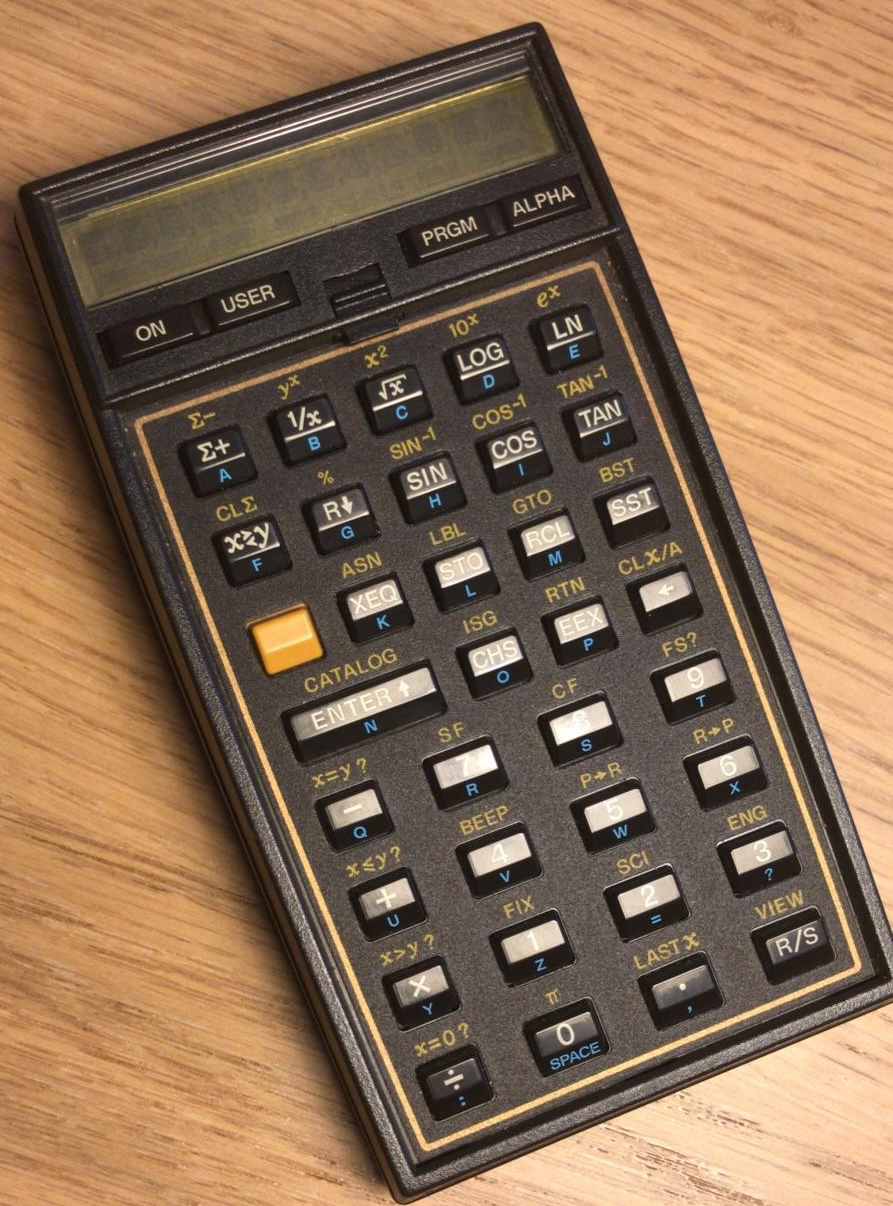
\includegraphics[width=\columnwidth]
			{fig-HP-41CV.jpg}
			{\tiny 
				HP-41CV,\\ 
				RPN Calculator,\\ 
				1979-1990\\
			}
	\end{column} % ++++ A
	\end{columns} % <<<<
\end{frame}
% ~~~~~~~~~~~~~~~~~~~~~~~~~~~~~~~~~~~~~~ A




%% ~~~~~~~~~~~~~~~~~~~~~~~~~~~~~~~~~~~~~~ V
%\begin{frame}\frametitle{RPN Evaluation}
%	\hCodeOutput{code-stack-RPN_Evaluator}[3.5][2.5]
%\end{frame}
%% ~~~~~~~~~~~~~~~~~~~~~~~~~~~~~~~~~~~~~~ A



% ~~~~~~~~~~~~~~~~~~~~~~~~~~~~~~~~~~~~~~ V
\hSubsection{Applications}{Infix to postfix conversion}{}
% ~~~~~~~~~~~~~~~~~~~~~~~~~~~~~~~~~~~~~~ A




% ~~~~~~~~~~~~~~~~~~~~~~~~~~~~~~~~~~~~~~ V
\begin{frame}\frametitle{Infix to postfix conversion}
	\begin{columns}[T] % >>>>
	\begin{column}{.5\linewidth} % ++++ V
	    	Use two stacks
		\begin{itemize}
			\item
			operator stack
			\item
			output stack
		\end{itemize}
	\end{column} % ++++ A
	\begin{column}{.7\linewidth} % ++++ V
	
			\vspace{-0.8cm}
{\small 
{\tt %mono space
\begin{center}
\begin{tabular}{|l|l|l|}
\hline
%\textbf{Input String} &\textbf{Output Stack} &\textbf{Operator Stack}\\
\textbf{Input } &\textbf{Stack} &\textbf{Stack}\\
\textbf{String} &\textbf{Output} &\textbf{Operator}\\
\hline
(f-e)/c*b+a & &(\\
(f-e)/c*b+a &f &(\\
(f-e)/c*b+a &f &(-\\
(f-e)/c*b+a &fe &(-\\
(f-e)/c*b+a &fe- &\\
(f-e)/c*b+a &fe- &/\\
(f-e)/c*b+a &fe-c &/\\
(f-e)/c*b+a &fe-c/ &*\\
(f-e)/c*b+a &fe-c/b &*\\
(f-e)/c*b+a &fe-c/b* &+\\
(f-e)/c*b+a &fe-c/b*a &+\\
(f-e)/c*b+a &fe-c/b*a+ &\\
\hline
\end{tabular}
\end{center}
}}

	\end{column} % ++++ A
	\end{columns} % <<<<
\end{frame}
% ~~~~~~~~~~~~~~~~~~~~~~~~~~~~~~~~~~~~~~ A



% ~~~~~~~~~~~~~~~~~~~~~~~~~~~~~~~~~~~~~~ V
\hSubsection{Applications}{Infix evaluation}{}
% ~~~~~~~~~~~~~~~~~~~~~~~~~~~~~~~~~~~~~~ A



% ~~~~~~~~~~~~~~~~~~~~~~~~~~~~~~~~~~~~~~ V
\begin{frame}\frametitle{Infix Evaluation}
	\begin{columns}[T] % >>>>
	\begin{column}{.5\linewidth} % ++++ V
{\tiny 
\begin{algorithm}[H]
	\SetKwData{StackOperand}{\texttt{stackOperand}}
	\SetKwData{StackOperator}{\texttt{stackOperator}}
	\SetKwData{Op}{\texttt{op}}
%    \KwData{infix algebraic expression}
%    \KwResult{value of the expression}
    \Begin{
 	\If{a number is read}
		 {Push it on the \StackOperand}
	\ElseIf{a ``(``  is read}
		{Push it on the \StackOperator}
	\ElseIf{operator \Op is read} {
		\While{the top of \StackOperator has a higher precedence than \Op}{
			Evaluate the top
		}
		Push \Op on \StackOperator
	}		
	\ElseIf {a ``)'' is read}{
		\While {the top of \StackOperator is not a ``(''}{
			Evaluate the top. 
		}
		Pop the ``(''
	}
	\ElseIf {there is no more input}{
		\While {the \StackOperator is not empty}{
			Evaluate the top
		}
	}
	Pop and display the result
    \caption{{\footnotesize Infix Evaluation}}
    }
\end{algorithm}
}

\hCite{Horstmann~\cite{horstmann2016big}}

	\end{column} % ++++ A
	\begin{column}{.5\linewidth} % ++++ V
	
	\vspace{-1.2cm}
\begin{center}
{\tiny
	expression: $(3+4)*(5-6)$\\
	
\begingroup
\setlength{\tabcolsep}{3pt}
\renewcommand{\arraystretch}{.2}
	\begin{tabular}{l l l}
		%
		\textbf{ch}
		&\textbf{stackOperand}
		&\textbf{stackOperator}\\
		%		
		(
		&\begin{tikzpicture}
			\hStack{0}{4}{-1}{} [0.5][0.4]
		\end{tikzpicture}
		&\begin{tikzpicture}
			\hStack{0}{4}{0}{``(''} [0.5][0.4]
		\end{tikzpicture}\\			
		%
		3
		&\begin{tikzpicture}
			\hStack{0}{4}{0}{3} [0.5][0.4]
		\end{tikzpicture}
		&\begin{tikzpicture}
			\hStack{0}{4}{0}{``(''} [0.5][0.4]
		\end{tikzpicture}\\	
		%
		+
		&\begin{tikzpicture}
			\hStack{0}{4}{0}{3} [0.5][0.4]
		\end{tikzpicture}
		&\begin{tikzpicture}
			\hStack{0}{4}{1}{``('', +} [0.5][0.4]
		\end{tikzpicture}\\	
		%
		4
		&\begin{tikzpicture}
			\hStack{0}{4}{1}{3, 4} [0.5][0.4]
		\end{tikzpicture}
		&\begin{tikzpicture}
			\hStack{0}{4}{1}{``('', +} [0.5][0.4]
		\end{tikzpicture}\\	
		%
		)
		&\begin{tikzpicture}
			\hStack{0}{4}{0}{7} [0.5][0.4]
		\end{tikzpicture}
		&\begin{tikzpicture}
			\hStack{0}{4}{-1}{} [0.5][0.4]
		\end{tikzpicture}\\	
		%
		*
		&\begin{tikzpicture}
			\hStack{0}{4}{0}{7} [0.5][0.4]
		\end{tikzpicture}
		&\begin{tikzpicture}
			\hStack{0}{4}{0}{*} [0.5][0.4]
		\end{tikzpicture}\\	
		%
		(
		&\begin{tikzpicture}
			\hStack{0}{4}{0}{7} [0.5][0.4]
		\end{tikzpicture}
		&\begin{tikzpicture}
			\hStack{0}{4}{1}{*, ``(''} [0.5][0.4]
		\end{tikzpicture}\\	
		%
		5
		&\begin{tikzpicture}
			\hStack{0}{4}{1}{7, 5} [0.5][0.4]
		\end{tikzpicture}
		&\begin{tikzpicture}
			\hStack{0}{4}{1}{*, ``(''} [0.5][0.4]
		\end{tikzpicture}\\	
		%
		$-$
		&\begin{tikzpicture}
			\hStack{0}{4}{1}{7, 5} [0.5][0.4]
		\end{tikzpicture}
		&\begin{tikzpicture}
			\hStack{0}{4}{2}{*, ``('', $-$} [0.5][0.4]
		\end{tikzpicture}\\
		%
		6
		&\begin{tikzpicture}
			\hStack{0}{4}{2}{7, 5, 6} [0.5][0.4]
		\end{tikzpicture}
		&\begin{tikzpicture}
			\hStack{0}{4}{2}{*, ``('', $-$} [0.5][0.4]
		\end{tikzpicture}\\	
		%
		)
		&\begin{tikzpicture}
			\hStack{0}{4}{1}{7, $-1$} [0.5][0.4]
		\end{tikzpicture}
		&\begin{tikzpicture}
			\hStack{0}{4}{0}{*} [0.5][0.4]
		\end{tikzpicture}\\	
		%
		~
		&\begin{tikzpicture}
			\hStack{0}{4}{0}{-7} [0.5][0.4]
		\end{tikzpicture}
		&\begin{tikzpicture}
			\hStack{0}{4}{-1}{} [0.5][0.4]
		\end{tikzpicture}\\	
		%
		~
		&\begin{tikzpicture}
			\hStack{0}{4}{-1}{} [0.5][0.4]
		\end{tikzpicture}
		&\begin{tikzpicture}
			\hStack{0}{4}{-1}{} [0.5][0.4]
		\end{tikzpicture}~~~
		\hEmph{{\small -7}}\\
		
	\end{tabular}
	\endgroup

}
\end{center}
	\end{column} % ++++ A
	\end{columns} % <<<<
\end{frame}
% ~~~~~~~~~~~~~~~~~~~~~~~~~~~~~~~~~~~~~~ A




% ~~~~~~~~~~~~~~~~~~~~~~~~~~~~~~~~~~~~~~ V
\hSubsection{Applications}{Backtracking}{}
% ~~~~~~~~~~~~~~~~~~~~~~~~~~~~~~~~~~~~~~ A




% ~~~~~~~~~~~~~~~~~~~~~~~~~~~~~~~~~~~~~~ V
\begin{frame}\frametitle{Decision Tree}
	\begin{columns}[T] % >>>>
	\begin{column}{.5\linewidth} % ++++ V
{\footnotesize  
\begin{itemize}
	
	\item 
	At a decision point, select one path, push the unselected paths to stack.
	
	\item 
	If a path unsuccessfully ends, pop the stack for a new path.
	
	\item 
	Keep doing as long as there is untested path in the stack.
	
\end{itemize}
}

	
\begin{tikzpicture} [level distance=10mm,
every node/.style={fill=red!25,circle,inner sep=1pt},
level 1/.style={sibling distance=20mm,nodes={fill=red!25}}, 
level 2/.style={sibling distance=10mm,nodes={fill=red!25}}, 
level 3/.style={sibling distance=5mm,nodes={fill=red!25}}]
	\node {1}
	child {
		node {2}
		child {
			node {4}
			child {
				node {8}
			}
			child[missing]
		}
		child {
			node {5}
			child {
				node {10}
			}
			child[missing]
		}
	}
	child {
		node {3}
		child {
			node {6}
			child[missing]
			child {
				node {13}
			}
		}
		child {
			node {7}
		}
	};
\end{tikzpicture}
	\end{column} % ++++ A
	\begin{column}{.5\linewidth} % ++++ V

\vspace{-1cm}
{\tiny
\begin{center}
%	expression: (~)~(~(~(~)~(~)~)~)\\
	\begin{tabular}{l l}
		\textbf{node}
		&\textbf{stack}\\
		
		1
		&\begin{tikzpicture}
			\hStack{0}{4}{-1}{} [0.5][0.5]
		\end{tikzpicture}\\			
		
		2
		&\begin{tikzpicture}
			\hStack{0}{4}{0}{3} [0.5][0.5]
		\end{tikzpicture}\\			
		
		4
		&\begin{tikzpicture}
			\hStack{0}{4}{1}{3, 5} [0.5][0.5]
		\end{tikzpicture}\\			
		
		8
		&\begin{tikzpicture}
			\hStack{0}{4}{1}{3, 5} [0.5][0.5]
		\end{tikzpicture}\\			
		% leaf
		
		5
		&\begin{tikzpicture}
			\hStack{0}{4}{0}{3} [0.5][0.5]
		\end{tikzpicture}\\			
		
		10
		&\begin{tikzpicture}
			\hStack{0}{4}{0}{3} [0.5][0.5]
		\end{tikzpicture}\\			
		% leaf
		
		3
		&\begin{tikzpicture}
			\hStack{0}{4}{-1}{} [0.5][0.5]
		\end{tikzpicture}\\			
		
		6
		&\begin{tikzpicture}
			\hStack{0}{4}{0}{7} [0.5][0.5]
		\end{tikzpicture}\\			
		
		13
		&\begin{tikzpicture}
			\hStack{0}{4}{0}{7} [0.5][0.5]
		\end{tikzpicture}\\			
		% leaf
		
		7
		&\begin{tikzpicture}
			\hStack{0}{4}{-1}{} [0.5][0.5]
		\end{tikzpicture}\\			

	\end{tabular}
\end{center}
} % \tiny
	\end{column} % ++++ A
	\end{columns} % <<<<
\end{frame}
% ~~~~~~~~~~~~~~~~~~~~~~~~~~~~~~~~~~~~~~ A




% ~~~~~~~~~~~~~~~~~~~~~~~~~~~~~~~~~~~~~~ V
\begin{frame}\frametitle{Web resources}
	\begin{itemize}

		\item 
		Problem Solving with Algorithms and Data Structures using Python
		\begin{itemize}
			
			\item 
			Home~\cite{pswads}
		
			\item 
			Infix, Prefix and Postfix Expressions~\cite{pswadsPostfix}
			
			\item
			What is a Stack~\cite{pswadsStack} 
			
		\end{itemize}

		\item 
		The Java Tutorials by Oracle
		\begin{itemize}
			
			\item 
			Home~\cite{TheJavaTutorials}
			
			\item
			Arrays~\cite{TheJavaTutorialsArray}
			
			\item
			Generics~\cite{TheJavaTutorialsGenerics}
			
		\end{itemize}
		
		\item
		HP Calculators (An RPN Calculator)
		\begin{itemize}
			
			\item 
			\hCite{
				\href
					{https://hp15c.com/web/hp15c.html}
					{HP-15 calculator online}~\cite{hp15online}
			}
		\end{itemize}
	\end{itemize}
\end{frame}
% ~~~~~~~~~~~~~~~~~~~~~~~~~~~~~~~~~~~~~~ A



% ~~~~~~~~~~~~~~~~~~~~~~~~~~~~~~~~~~~~~~ V
\hSection[Idea]{The Idea of a Stack}
% ~~~~~~~~~~~~~~~~~~~~~~~~~~~~~~~~~~~~~~ A

% ~~~~~~~~~~~~~~~~~~~~~~~~~~~~~~~~~~~~~~ V
\subsection[LIFO]{Last in, first out}
% ~~~~~~~~~~~~~~~~~~~~~~~~~~~~~~~~~~~~~~ A




% ~~~~~~~~~~~~~~~~~~~~~~~~~~~~~~~~~~~~~~ V frm
\begin{frame}[t,fragile] \frametitle{A stack of plates}
  \begin{columns}[T]
    \begin{column}{0.42\textwidth}
      \begin{center}
      \begin{tikzpicture}[plate/.style={draw, thick, rounded corners=2pt, minimum width=2.6cm, minimum height=0.45cm, font=\small}]
        \node[plate, fill=red!25]   (a) at (0,0)    {A (first in)};
        \node[plate, fill=red!25]   (b) at (0,0.5)  {B};
        \node[plate, fill=red!25]   (c) at (0,1.0)  {C};
        \node[plate, fill=green!40] (d) at (0,1.5)  {D (last in)};
        \draw[thick] (-1.6,-0.3) -- (1.6,-0.3);
        \draw[-latex, very thick, blue] (-1.7,2.8) node[left, font=\small] {push} to[bend right=30] (-0.9,1.85);
        \draw[-latex, very thick, orange] (0.9,1.85) to[bend right=30] (1.7,2.8) node[right, font=\small] {pop};
        \node[font=\small, red] at (1.95,1.5) {$\leftarrow$ top};
      \end{tikzpicture}
      \end{center}
    \end{column}
    \begin{column}{0.54\textwidth}
      \begin{itemize}
        \item You can only put a plate \textbf{on top} (\emph{push}).
        \item You can only take the plate \textbf{on top} (\emph{pop}).
        \item The plate put last is taken first:\\
          \hRemark{LIFO: Last In, First Out}.
        \item The plates below the top cannot be reached until the ones above are removed.
      \end{itemize}
      \begin{block}{Definition}
        A \textbf{stack} is a collection where insertion and removal happen at one end only, called the \textbf{top}.
      \end{block}
    \end{column}
  \end{columns}
\end{frame}
% ~~~~~~~~~~~~~~~~~~~~~~~~~~~~~~~~~~~~~~ A frm




% ~~~~~~~~~~~~~~~~~~~~~~~~~~~~~~~~~~~~~~ V frm
\begin{frame}[t,fragile] \frametitle{Stacks around us}
  \begin{center}\small
  \begin{tabular}{L{0.26\textwidth}L{0.3\textwidth}L{0.34\textwidth}}
    \toprule
    \textbf{Where}           & \textbf{push}                 & \textbf{pop} \\
    \midrule
    Undo in an editor        & every change you make         & \keys{Ctrl+Z} (\win) / \keys{\cmd+Z} (\mac) \\
    Back button of a browser & every page you open           & \emph{Back} \\
    Function calls           & calling a method              & returning from it \\
    Checking brackets        & an opening \texttt{(} \texttt{[} \texttt{\{} & the matching closing one \\
    A maze, depth first      & a new corridor                & a dead end: go back \\
    \bottomrule
  \end{tabular}
  \end{center}
  \vspace{0.5em}
  In each case the \textbf{most recent} unfinished thing is handled first.
\end{frame}
% ~~~~~~~~~~~~~~~~~~~~~~~~~~~~~~~~~~~~~~ A frm




% ~~~~~~~~~~~~~~~~~~~~~~~~~~~~~~~~~~~~~~ V frm
\begin{frame}[t,fragile] \frametitle{Stack vs queue}
  \begin{columns}[T]
    \begin{column}{0.48\textwidth}
      \begin{block}{Stack: LIFO}
        \begin{center}
        \begin{tikzpicture}\hStack{0}{6}{3}{A,B,C,D}[0.6][0.5]\end{tikzpicture}
        \end{center}
        \small Insert and remove at the \textbf{same} end (the top). \texttt{pop} gives \textbf{D}.
      \end{block}
    \end{column}
    \begin{column}{0.48\textwidth}
      \begin{block}{Queue: FIFO}
        \begin{center}
        \begin{tikzpicture}\hQueue{0}{6}{0}{4}{A,B,C,D}[0.6][0.5]\end{tikzpicture}
        \end{center}
        \small Insert at the tail, remove at the head. \texttt{dequeue} gives \textbf{A}.
      \end{block}
    \end{column}
  \end{columns}
  \vspace{0.5em}
  \small Same elements, same order of arrival, \hRemark{opposite order of leaving}.
\end{frame}
% ~~~~~~~~~~~~~~~~~~~~~~~~~~~~~~~~~~~~~~ A frm

% ~~~~~~~~~~~~~~~~~~~~~~~~~~~~~~~~~~~~~~ V
\hSection[ADT]{The Stack ADT}
% ~~~~~~~~~~~~~~~~~~~~~~~~~~~~~~~~~~~~~~ A

% ~~~~~~~~~~~~~~~~~~~~~~~~~~~~~~~~~~~~~~ V
\subsection[Operations]{Operations}
% ~~~~~~~~~~~~~~~~~~~~~~~~~~~~~~~~~~~~~~ A




% ~~~~~~~~~~~~~~~~~~~~~~~~~~~~~~~~~~~~~~ V frm
\begin{frame}[t,fragile] \frametitle{What a stack can do}
  \begin{center}\small
  \begin{tabular}{lL{0.42\textwidth}L{0.3\textwidth}}
    \toprule
    \textbf{Operation}          & \textbf{Meaning}                                 & \textbf{If the stack is \dots} \\
    \midrule
    \texttt{push(x)}            & put \texttt{x} on top                            & full: \hRemark{overflow} \\
    \texttt{pop()}              & remove the top element and return it             & empty: \hRemark{underflow} \\
    \texttt{peek()}             & return the top element, do not remove it         & empty: \hRemark{underflow} \\
    \texttt{isEmpty()}          & is there no element?                             & -- \\
    \texttt{size()}             & number of elements                               & -- \\
    \bottomrule
  \end{tabular}
  \end{center}
  \vspace{0.5em}
  \begin{itemize}\small
    \item This list is an \textbf{abstract data type} (ADT): it says \emph{what} a stack does, not \emph{how}.
    \item \texttt{peek} is also called \texttt{top}. Overflow only happens if the capacity is fixed.
  \end{itemize}
\end{frame}
% ~~~~~~~~~~~~~~~~~~~~~~~~~~~~~~~~~~~~~~ A frm




% ~~~~~~~~~~~~~~~~~~~~~~~~~~~~~~~~~~~~~~ V frm
\begin{frame}[t,fragile] \frametitle{Rules every stack obeys}
  For any stack $S$ and element $x$:
%  \[
%  	\hCode{peek({push}(S, x)) = x}
%%  	\mathrm{peek}(\mathrm{push}(S, x)) = x
%  \]
%  \[
%  	\mathrm{pop}(\mathrm{push}(S, x)) \text{ returns } x \text{ and leaves } S
%  \]
%  \[
%  	\mathrm{size}(\mathrm{push}(S, x)) = \mathrm{size}(S) + 1
%  \]
%  \[
%  	\mathrm{isEmpty}(S) \iff \mathrm{size}(S) = 0
%  \]
  \[
  	\hCode{peek({push}(S, x)) = x}
  \]
  \[
  	\hCode{pop({push}(S, x))} \text{ returns } x \text{ and leaves } S
  \]
  \[
  	\hCode{size({push}(S, x)) = {size}(S) + 1}
  \]
  \[
  	\hCode{isEmpty(S)} \iff \hCode{{size}(S) = 0}
  \]
  \vspace{0.3em}
  \begin{itemize}\small
    \item Any implementation (array, linked list, \dots) must make these true.
    \item They are also good \textbf{test cases}: push, then peek; push, then pop.
  \end{itemize}
\end{frame}
% ~~~~~~~~~~~~~~~~~~~~~~~~~~~~~~~~~~~~~~ A frm

% ~~~~~~~~~~~~~~~~~~~~~~~~~~~~~~~~~~~~~~ V
\subsection[Trace]{A trace}
% ~~~~~~~~~~~~~~~~~~~~~~~~~~~~~~~~~~~~~~ A




% ~~~~~~~~~~~~~~~~~~~~~~~~~~~~~~~~~~~~~~ V frm
\begin{frame}[t,fragile] \frametitle{Tracing a sequence of operations}
  \begin{columns}[T]
    \begin{column}{0.5\textwidth}
      \begin{center}\footnotesize
      \begin{tabular}{lll}
        \toprule
        \textbf{Operation} & \textbf{Returns} & \textbf{Stack (bottom $\to$ top)} \\
        \midrule
        \texttt{push(3)}  &                & 3 \\
        \texttt{push(7)}  &                & 3 7 \\
        \texttt{peek()}   & 7              & 3 7 \\
        \texttt{push(5)}  &                & 3 7 5 \\
        \texttt{pop()}    & 5              & 3 7 \\
        \texttt{pop()}    & 7              & 3 \\
        \texttt{size()}   & 1              & 3 \\
        \texttt{pop()}    & 3              & (empty) \\
        \texttt{pop()}    & \hRemark{underflow} & (empty) \\
        \bottomrule
      \end{tabular}
      \end{center}
    \end{column}
    \begin{column}{0.46\textwidth}
      \begin{block}{Try it}
        \small What does this return?\\[0.3em]
        \texttt{push(1); push(2); pop();}\\
        \texttt{push(3); push(4); pop(); pop();}
        \uncover<2->{\\[0.3em] \hRemark{4, then 3}; the stack holds \texttt{1}.}
      \end{block}
    \end{column}
  \end{columns}
\end{frame}
% ~~~~~~~~~~~~~~~~~~~~~~~~~~~~~~~~~~~~~~ A frm

% ~~~~~~~~~~~~~~~~~~~~~~~~~~~~~~~~~~~~~~ V
\hSection[Array]{Stack Using an Array}
% ~~~~~~~~~~~~~~~~~~~~~~~~~~~~~~~~~~~~~~ A

% ~~~~~~~~~~~~~~~~~~~~~~~~~~~~~~~~~~~~~~ V
\subsection[Idea]{Array and top}
% ~~~~~~~~~~~~~~~~~~~~~~~~~~~~~~~~~~~~~~ A




% ~~~~~~~~~~~~~~~~~~~~~~~~~~~~~~~~~~~~~~ V frm
\begin{frame}[t,fragile] \frametitle{An array and an index}
  \begin{columns}[T]
    \begin{column}{0.5\textwidth}
      \begin{itemize}
        \item an array \texttt{a} of capacity $n$
        \item an integer \texttt{top}: the index of the top element
        \item elements live in \texttt{a[0]} \dots{} \texttt{a[top]}
        \item empty stack: \texttt{top} $= -1$
        \item full stack: \texttt{top} $= n - 1$
      \end{itemize}
      \vspace{0.3em}
      \small The bottom of the stack is \texttt{a[0]} and never moves. Only \texttt{top} changes, so nothing is shifted.
    \end{column}
    \begin{column}{0.46\textwidth}
      \small empty, \texttt{top = -1}\\
      \begin{tikzpicture}\hStack{0}{6}{-1}{}[0.6][0.5]\end{tikzpicture}\\[0.4em]
      after \texttt{push(10)}, \texttt{push(20)}, \texttt{push(30)}: \texttt{top = 2}\\
      \begin{tikzpicture}\hStack{0}{6}{2}{10,20,30}[0.6][0.5]\end{tikzpicture}\\[0.4em]
      after \texttt{pop()} returns 30: \texttt{top = 1}\\
      \begin{tikzpicture}\hStack{0}{6}{1}{10,20}[0.6][0.5]\end{tikzpicture}\\[0.4em]
      full, \texttt{top = 5}\\
      \begin{tikzpicture}\hStack{0}{6}{5}{10,20,40,50,60,70}[0.6][0.5]\end{tikzpicture}
    \end{column}
  \end{columns}
\end{frame}
% ~~~~~~~~~~~~~~~~~~~~~~~~~~~~~~~~~~~~~~ A frm




% ~~~~~~~~~~~~~~~~~~~~~~~~~~~~~~~~~~~~~~ V frm
\begin{frame}[t,fragile] \frametitle{Two common conventions}
  \begin{center}\small
  \begin{tabular}{lll}
    \toprule
                            & \texttt{top} = index of the top     & \texttt{size} = number of elements \\
    \midrule
    empty                   & \texttt{top == -1}                  & \texttt{size == 0} \\
    full                    & \texttt{top == n - 1}               & \texttt{size == n} \\
    top element             & \texttt{a[top]}                     & \texttt{a[size - 1]} \\
    push                    & \texttt{a[++top] = x}               & \texttt{a[size++] = x} \\
    pop                     & \texttt{return a[top--]}            & \texttt{return a[--size]} \\
    \bottomrule
  \end{tabular}
  \end{center}
  \vspace{0.4em}
  \begin{itemize}\small
    \item Both are correct. Pick one and use it \textbf{everywhere}: mixing them gives off-by-one errors.
    \item \texttt{size} is popular in Java (\texttt{ArrayList} works this way). These slides use \texttt{top}, as in the figures.
    \item \hRemark{Watch} \texttt{++top} (increment, then use) versus \texttt{top++} (use, then increment).
  \end{itemize}
\end{frame}
% ~~~~~~~~~~~~~~~~~~~~~~~~~~~~~~~~~~~~~~ A frm

% ~~~~~~~~~~~~~~~~~~~~~~~~~~~~~~~~~~~~~~ V
\subsection[Algorithms]{Algorithms}
% ~~~~~~~~~~~~~~~~~~~~~~~~~~~~~~~~~~~~~~ A




% ~~~~~~~~~~~~~~~~~~~~~~~~~~~~~~~~~~~~~~ V frm
\begin{frame}[t,fragile] \frametitle{Push and pop}
  \begin{columns}[T]
    \begin{column}{0.49\textwidth}
      \SetAlFnt{\small}


% +++++++++++++++++++++++++++++++++++++++ V alg
%: -Alg. 
\begin{algorithm}[H]
  \caption{Push}
  \KwIn{stack $(a, top)$ of capacity $n$, element $x$}
  \If{$top = n - 1$}{\KwError{overflow}\;}
  $top \gets top + 1$\;
  $a[top] \gets x$\;
\end{algorithm}
% +++++++++++++++++++++++++++++++++++++++ A alg

    \end{column}
    \begin{column}{0.49\textwidth}
      \SetAlFnt{\small}


% +++++++++++++++++++++++++++++++++++++++ V alg
%: -Alg. 
\begin{algorithm}[H]
  \caption{Pop}
  \KwIn{stack $(a, top)$}
  \KwOut{the top element}
  \If{$top = -1$}{\KwError{underflow}\;}
  $x \gets a[top]$\;
  $top \gets top - 1$\;
  \Return{$x$}\;
\end{algorithm}
% +++++++++++++++++++++++++++++++++++++++ A alg

    \end{column}
  \end{columns}
  \small Each runs a \textbf{fixed} number of steps, whatever the size of the stack: $O(1)$.
\end{frame}
% ~~~~~~~~~~~~~~~~~~~~~~~~~~~~~~~~~~~~~~ A frm




% ~~~~~~~~~~~~~~~~~~~~~~~~~~~~~~~~~~~~~~ V frm
\begin{frame}[t,fragile] \frametitle{Peek, isEmpty, size}
  \begin{columns}[T]
    \begin{column}{0.49\textwidth}
      \SetAlFnt{\small}


% +++++++++++++++++++++++++++++++++++++++ V alg
%: -Alg. 
\begin{algorithm}[H]
  \caption{Peek}
  \KwIn{stack $(a, top)$}
  \KwOut{the top element, not removed}
  \If{$top = -1$}{\KwError{underflow}\;}
  \Return{$a[top]$}\;
\end{algorithm}
% +++++++++++++++++++++++++++++++++++++++ A alg

    \end{column}
    \begin{column}{0.49\textwidth}
      \SetAlFnt{\small}


% +++++++++++++++++++++++++++++++++++++++ V alg
%: -Alg. 
\begin{algorithm}[H]
  \caption{IsEmpty and Size}
  \KwIn{stack $(a, top)$}
  \Return{$top = -1$}\tcp*{isEmpty}
  \Return{$top + 1$}\tcp*{size}
\end{algorithm}
% +++++++++++++++++++++++++++++++++++++++ A alg

    \end{column}
  \end{columns}
  \small A popped element stays in the array, but it is no longer part of the stack: the next push overwrites it.
\end{frame}
% ~~~~~~~~~~~~~~~~~~~~~~~~~~~~~~~~~~~~~~ A frm

% ~~~~~~~~~~~~~~~~~~~~~~~~~~~~~~~~~~~~~~ V
\subsection[Errors]{Overflow and underflow}
% ~~~~~~~~~~~~~~~~~~~~~~~~~~~~~~~~~~~~~~ A




% ~~~~~~~~~~~~~~~~~~~~~~~~~~~~~~~~~~~~~~ V frm
\begin{frame}[t,fragile] \frametitle{When things go wrong}
  \begin{columns}[T]
    \begin{column}{0.48\textwidth}
      \begin{block}{Overflow: push on a full stack}
        \begin{tikzpicture}\hStack{0}{4}{3}{A,B,C,D}[0.6][0.5]\end{tikzpicture}\\[0.3em]
        \small There is no \texttt{a[4]}. Options:
        \begin{itemize}\small
          \item report an error (throw an exception)
          \item \textbf{grow}: copy into a bigger array
        \end{itemize}
      \end{block}
    \end{column}
    \begin{column}{0.48\textwidth}
      \begin{block}{Underflow: pop on an empty stack}
        \begin{tikzpicture}\hStack{0}{4}{-1}{}[0.6][0.5]\end{tikzpicture}\\[0.3em]
        \small There is no top element. Options:
        \begin{itemize}\small
          \item throw an exception (Java: \texttt{EmptyStackException}, \texttt{NoSuchElementException})
          \item return a special value (\texttt{null}): \texttt{ArrayDeque.poll()}
        \end{itemize}
      \end{block}
    \end{column}
  \end{columns}
  \vspace{0.3em}
  \small Without a check, Java stops the program with \texttt{ArrayIndexOutOfBoundsException}: the bug is found, but the message does not say ``stack''.
\end{frame}
% ~~~~~~~~~~~~~~~~~~~~~~~~~~~~~~~~~~~~~~ A frm

% ~~~~~~~~~~~~~~~~~~~~~~~~~~~~~~~~~~~~~~ V
\hSection[Growing]{A Stack That Grows}
% ~~~~~~~~~~~~~~~~~~~~~~~~~~~~~~~~~~~~~~ A




% ~~~~~~~~~~~~~~~~~~~~~~~~~~~~~~~~~~~~~~ V frm
\begin{frame}[t,fragile] \frametitle{Doubling the array}
  \begin{columns}[T]
    \begin{column}{0.5\textwidth}
      \small push \texttt{E} on a full stack of capacity 4:\\[0.2em]
      \begin{tikzpicture}\hStack{0}{4}{3}{A,B,C,D}[0.6][0.5]\end{tikzpicture}\\[0.3em]
      1. make an array of capacity 8, copy:\\[0.2em]
      \begin{tikzpicture}\hStack{0}{8}{3}{A,B,C,D}[0.6][0.5]\end{tikzpicture}\\[0.3em]
      2. push as usual:\\[0.2em]
      \begin{tikzpicture}\hStack{0}{8}{4}{A,B,C,D,E}[0.6][0.5]\end{tikzpicture}
    \end{column}
    \begin{column}{0.46\textwidth}
      \begin{itemize}\small
        \item Copying $k$ elements costs $k$ steps.
        \item It happens \textbf{rarely}: at sizes $1, 2, 4, 8, \dots$
        \item Grow by \textbf{doubling}, not by adding 1: adding 1 makes \emph{every} push copy the whole array.
      \end{itemize}
      \begin{block}{Java}
        \small \texttt{ArrayList} grows by about 1.5 times, \texttt{ArrayDeque} by 1.5 or 2 times, \texttt{Vector} (and \texttt{Stack}) by 2 times.
      \end{block}
    \end{column}
  \end{columns}
\end{frame}
% ~~~~~~~~~~~~~~~~~~~~~~~~~~~~~~~~~~~~~~ A frm




% ~~~~~~~~~~~~~~~~~~~~~~~~~~~~~~~~~~~~~~ V frm
\begin{frame}[t,fragile] \frametitle{Why doubling is cheap: amortized cost}
  Push $n$ elements into a stack that starts with capacity 1 and doubles when full.
  Copies happen at sizes $1, 2, 4, \dots, 2^{k}$ with $2^{k} < n$:
  \[
  	\text{copies} = 1 + 2 + 4 + \dots + 2^{k} = 2^{k+1} - 1 < 2n
  \]
  \[
  	\text{total work} < n + 2n = 3n
  \]
  \vspace{0.2em}
  \begin{itemize}
    \item So the \textbf{average} cost of one push is less than 3 steps: $O(1)$ \hRemark{amortized}.
    \item A single push can still cost $O(n)$ (the one that copies).
    \item Growing by a constant amount $c$ instead costs about $\frac{n^{2}}{2c}$ copies: $O(n)$ per push.
    \item Shrinking: halve the array when it is only \textbf{one quarter} full (not half full), so a push/pop sequence at the boundary does not copy every time.
  \end{itemize}
\end{frame}
% ~~~~~~~~~~~~~~~~~~~~~~~~~~~~~~~~~~~~~~ A frm

% ~~~~~~~~~~~~~~~~~~~~~~~~~~~~~~~~~~~~~~ V
\hSection[Cost]{Cost of the Operations}
% ~~~~~~~~~~~~~~~~~~~~~~~~~~~~~~~~~~~~~~ A




% ~~~~~~~~~~~~~~~~~~~~~~~~~~~~~~~~~~~~~~ V frm
\begin{frame}[t,fragile] \frametitle{Running time and memory}
  \begin{center}\small
  \begin{tabular}{lccc}
    \toprule
    \textbf{Operation} & \textbf{fixed array} & \textbf{growing array} & \textbf{linked list} \\
    \midrule
    \texttt{push}      & $O(1)$               & $O(1)$ amortized, $O(n)$ worst & $O(1)$ \\
    \texttt{pop}       & $O(1)$               & $O(1)$ amortized               & $O(1)$ \\
    \texttt{peek}, \texttt{isEmpty}, \texttt{size} & $O(1)$ & $O(1)$          & $O(1)$ \\
    memory             & capacity $n$         & between $n$ and $4n$ slots     & $n$ nodes, each with a link \\
    limit              & overflow             & only the memory               & only the memory \\
    \bottomrule
  \end{tabular}
  \end{center}
  \vspace{0.4em}
  \begin{itemize}\small
    \item Arrays keep elements \textbf{next to each other} in memory: fast for the processor's cache.
    \item Linked lists need one extra object per element: more memory, more work for the garbage collector.
    \item Java's \texttt{ArrayDeque} is a growing array. Which is faster depends on the use: \textbf{measure} (junior deck).
  \end{itemize}
\end{frame}
% ~~~~~~~~~~~~~~~~~~~~~~~~~~~~~~~~~~~~~~ A frm

% ~~~~~~~~~~~~~~~~~~~~~~~~~~~~~~~~~~~~~~ V
\hSection[Applications]{Applications}
% ~~~~~~~~~~~~~~~~~~~~~~~~~~~~~~~~~~~~~~ A

% ~~~~~~~~~~~~~~~~~~~~~~~~~~~~~~~~~~~~~~ V
\subsection[Brackets]{Balanced brackets}
% ~~~~~~~~~~~~~~~~~~~~~~~~~~~~~~~~~~~~~~ A




% ~~~~~~~~~~~~~~~~~~~~~~~~~~~~~~~~~~~~~~ V frm
\begin{frame}[t,fragile] \frametitle{Are the brackets balanced?}
  \begin{columns}[T]
    \begin{column}{0.56\textwidth}
      \SetAlFnt{\small}


% +++++++++++++++++++++++++++++++++++++++ V alg
%: -Alg. 
\begin{algorithm}[H]
  \caption{Balanced}
  \KwIn{a string $w$}
  \KwOut{true if every bracket is closed in order}
  $S \gets$ empty stack\;
  \ForEach{character $c$ of $w$}{
    \uIf{$c$ is \texttt{(} or \texttt{[} or \texttt{\{}}{push $c$ onto $S$\;}
    \ElseIf{$c$ is \texttt{)} or \texttt{]} or \texttt{\}}}{
      \lIf{$S$ is empty}{\Return{false}}
      \lIf{pop($S$) does not match $c$}{\Return{false}}
    }
  }
  \Return{$S$ is empty}\;
\end{algorithm}
% +++++++++++++++++++++++++++++++++++++++ A alg

    \end{column}
    \begin{column}{0.4\textwidth}
      \small
      \begin{tabular}{ll}
        \toprule
        \textbf{input} & \textbf{result} \\
        \midrule
        \texttt{(a[i] + b)}   & balanced \\
        \texttt{\{ [ ( ) ] \}} & balanced \\
        \texttt{( ]}          & mismatch \\
        \texttt{( ( )}        & left open \\
        \texttt{) (}          & nothing to close \\
        \bottomrule
      \end{tabular}
      \vspace{0.4em}

      Compilers do this for every program you write.
    \end{column}
  \end{columns}
\end{frame}
% ~~~~~~~~~~~~~~~~~~~~~~~~~~~~~~~~~~~~~~ A frm

% ~~~~~~~~~~~~~~~~~~~~~~~~~~~~~~~~~~~~~~ V
\subsection[Postfix]{Postfix expressions}
% ~~~~~~~~~~~~~~~~~~~~~~~~~~~~~~~~~~~~~~ A




% ~~~~~~~~~~~~~~~~~~~~~~~~~~~~~~~~~~~~~~ V frm
\begin{frame}[t,fragile] \frametitle{Evaluating a postfix expression}
  \begin{columns}[T]
    \begin{column}{0.48\textwidth}
      Infix \texttt{(3 + 4) * 2} is \textbf{postfix} \texttt{3 4 + 2 *}: the operator comes after its operands, no brackets needed.
      \begin{itemize}\small
        \item number: push it
        \item operator: pop $b$, pop $a$, push $a \text{ op } b$
        \item at the end, the stack holds the result
      \end{itemize}
      \small Used by calculators (HP, ``RPN''), by the Java virtual machine, and by PostScript.
    \end{column}
    \begin{column}{0.48\textwidth}
      \begin{center}\small
      \begin{tabular}{lll}
        \toprule
        \textbf{token} & \textbf{action}     & \textbf{stack} \\
        \midrule
        \texttt{3}     & push                & 3 \\
        \texttt{4}     & push                & 3 4 \\
        \texttt{+}     & $3 + 4$             & 7 \\
        \texttt{2}     & push                & 7 2 \\
        \texttt{*}     & $7 \times 2$        & 14 \\
        \bottomrule
      \end{tabular}
      \end{center}
      \small \hRemark{Order matters}: for \texttt{-} and \texttt{/} the \emph{second} pop is the left operand.
    \end{column}
  \end{columns}
\end{frame}
% ~~~~~~~~~~~~~~~~~~~~~~~~~~~~~~~~~~~~~~ A frm

% ~~~~~~~~~~~~~~~~~~~~~~~~~~~~~~~~~~~~~~ V
\subsection[Calls]{The call stack}
% ~~~~~~~~~~~~~~~~~~~~~~~~~~~~~~~~~~~~~~ A




% ~~~~~~~~~~~~~~~~~~~~~~~~~~~~~~~~~~~~~~ V frm
\begin{frame}[t,fragile] \frametitle{Method calls use a stack}
  \begin{columns}[T]
    \begin{column}{0.4\textwidth}
      \begin{center}
      \begin{tikzpicture}[fr/.style={draw, thick, minimum width=3.6cm, minimum height=0.55cm, font=\ttfamily\small}]
        \node[fr, fill=gray!15]   at (0,0)    {main(args)};
        \node[fr, fill=red!20]    at (0,0.6)  {fact(n = 3)};
        \node[fr, fill=red!20]    at (0,1.2)  {fact(n = 2)};
        \node[fr, fill=green!35]  at (0,1.8)  {fact(n = 1)};
        \node[font=\small, red] at (2.5,1.8) {$\leftarrow$ top};
        \draw[thick] (-1.9,-0.35) -- (1.9,-0.35);
      \end{tikzpicture}
      \end{center}
    \end{column}
    \begin{column}{0.56\textwidth}
      \begin{itemize}\small
        \item Each call \textbf{pushes} a frame: its parameters, local variables and where to return.
        \item Each \texttt{return} \textbf{pops} the frame and continues the caller.
        \item Recursion that never stops fills it up: Java throws \texttt{StackOverflowError}.
        \item An exception's \emph{stack trace} is this stack, printed from the top.
      \end{itemize}
    \end{column}
  \end{columns}
\end{frame}
% ~~~~~~~~~~~~~~~~~~~~~~~~~~~~~~~~~~~~~~ A frm




% ~~~~~~~~~~~~~~~~~~~~~~~~~~~~~~~~~~~~~~ V frm
\begin{frame}[t,fragile] \frametitle{More uses}
  \begin{itemize}
    \item \textbf{Undo / redo}: two stacks. Undo pops from \emph{undo} and pushes onto \emph{redo}; a new edit clears \emph{redo}.
    \item \textbf{Reversing}: push all, pop all: \texttt{"stack"} becomes \texttt{"kcats"}.
    \item \textbf{Depth-first search}: in a maze or a graph, the stack holds the path still to explore.
    \item \textbf{Infix to postfix}: Dijkstra's \emph{shunting-yard} algorithm keeps operators on a stack.
    \item \textbf{Backtracking}: sudoku, the 8 queens: undo the last choice when stuck.
    \item \textbf{Number conversion}: decimal to binary, remainders come out in reverse.
  \end{itemize}
\end{frame}
% ~~~~~~~~~~~~~~~~~~~~~~~~~~~~~~~~~~~~~~ A frm

% ~~~~~~~~~~~~~~~~~~~~~~~~~~~~~~~~~~~~~~ V
\hSection[Java]{Stacks in Java}
% ~~~~~~~~~~~~~~~~~~~~~~~~~~~~~~~~~~~~~~ A




% ~~~~~~~~~~~~~~~~~~~~~~~~~~~~~~~~~~~~~~ V frm
\begin{frame}[t,fragile] \frametitle{Which class?}
  \begin{center}\small
  \begin{tabular}{lL{0.24\textwidth}L{0.42\textwidth}}
    \toprule
    \textbf{Class}                 & \textbf{Since}    & \textbf{Note} \\
    \midrule
    \hCode{java.util.Stack}       & Java 1.0 (1996)   & extends \texttt{Vector}: synchronized, also allows \hCode{get(i)}, \hCode{add(i, x)} \\
    \hCode{java.util.ArrayDeque}  & Java 6 (2006)     & \hRemark{recommended}: a growing array, \hCode{push}, \hCode{pop}, \hCode{peek} \\
    \hCode{java.util.LinkedList}  & Java 1.2          & also a \texttt{Deque}; a linked list \\
    your own \texttt{ArrayStack}   &                   & to learn how it works (next decks) \\
    \bottomrule
  \end{tabular}
  \end{center}
  \vspace{0.3em}

  \small The Java documentation of \texttt{Stack} says: ``A more complete and consistent set of LIFO stack operations is provided by the
  \texttt{Deque} interface and its implementations, which should be used in preference to this class.''
\end{frame}
% ~~~~~~~~~~~~~~~~~~~~~~~~~~~~~~~~~~~~~~ A frm




% ~~~~~~~~~~~~~~~~~~~~~~~~~~~~~~~~~~~~~~ V frm
\begin{frame}[t,fragile] \frametitle{Trying it: \texttt{jshell}}
  \small Open a terminal (\win: \emph{Command Prompt}; \mac: \emph{Terminal}) and type \texttt{jshell}.
  The same lines, saved as \texttt{try.jsh}:
  \lstcode[basicstyle=\ttfamily\tiny, numbers=none]{codeoutput/JShell/try.jsh}{Java}

  \lstterminal[basicstyle=\ttfamily\footnotesize]{codeoutput/JShell.txt}

  \vspace{0.1em}
  \small
  \texttt{ArrayDeque} prints from the \textbf{top}: \texttt{[30, 20, 10]}. (\texttt{java.util.Stack} prints from the bottom.)
\end{frame}
% ~~~~~~~~~~~~~~~~~~~~~~~~~~~~~~~~~~~~~~ A frm

% ~~~~~~~~~~~~~~~~~~~~~~~~~~~~~~~~~~~~~~ V
\hSection[Summary]{Summary}
% ~~~~~~~~~~~~~~~~~~~~~~~~~~~~~~~~~~~~~~ A




% ~~~~~~~~~~~~~~~~~~~~~~~~~~~~~~~~~~~~~~ V frm
\begin{frame}[t,fragile] \frametitle{Big ideas}
  \begin{itemize}
    \item A stack is \textbf{LIFO}: insert and remove at the top only.
    \item ADT: \texttt{push}, \texttt{pop}, \texttt{peek}, \texttt{isEmpty}, \texttt{size}; errors are \emph{overflow} and \emph{underflow}.
    \item With an array: elements in \texttt{a[0..top]}, \texttt{top = -1} when empty; nothing ever moves.
    \item Every operation is $O(1)$; a growing array doubles its capacity, $O(1)$ amortized.
    \item Uses: undo, brackets, postfix, method calls, depth-first search, backtracking.
    \item In Java use \texttt{ArrayDeque} (not the old \texttt{Stack}); write your own to understand it.
  \end{itemize}
\end{frame}
% ~~~~~~~~~~~~~~~~~~~~~~~~~~~~~~~~~~~~~~ A frm




% ~~~~~~~~~~~~~~~~~~~~~~~~~~~~~~~~~~~~~~ V frm
\begin{frame}[t,fragile] \frametitle{Check yourself}
  \begin{enumerate}\small
    \item After \texttt{push(1), push(2), pop(), push(3), peek()}, what is returned and what is left?
    \item An array stack has capacity 5 and \texttt{top = 4}. What happens on \texttt{push}? And with \texttt{top = -1} on \texttt{pop}?
    \item Why does a growing stack double its array instead of adding one slot?
    \item Evaluate the postfix expression \texttt{5 1 2 + 4 * + 3 -}.
    \item Which brackets are wrong in \texttt{\{ ( [ ] ) ( \}}? Trace the stack.
    \item Why is \texttt{ArrayDeque} preferred to \texttt{java.util.Stack}?
  \end{enumerate}
\end{frame}
% ~~~~~~~~~~~~~~~~~~~~~~~~~~~~~~~~~~~~~~ A frm




% ~~~~~~~~~~~~~~~~~~~~~~~~~~~~~~~~~~~~~~ V frm
\begin{frame}[t,fragile]
	\begin{center}
		\vspace{4cm}
		\hRemark{\Huge Questions?}
	\end{center}
\end{frame}
% ~~~~~~~~~~~~~~~~~~~~~~~~~~~~~~~~~~~~~~ A frm



\end{document}
